\documentclass[a4paper]{article}


% import packages
\usepackage{graphicx}  % for \includegraphics with jpg,png,...
\usepackage[english,ngerman]{isodate, babel}  % ngerman: Neue Rechtschreibung
\usepackage{url}
\usepackage[dvipsnames]{xcolor}  % for \color
\usepackage{listings}  % source code support
\usepackage[T1]{fontenc}
\usepackage[utf8]{inputenc}
\usepackage{textcomp}  % support for symbols like €
\usepackage{lmodern}  % improve font
\usepackage{float}  % allow H option in \begin{subfigure}[H]
\usepackage{caption}
\usepackage{hyperref}
\usepackage{subcaption}
\usepackage[%
backend=biber,
sortlocale=de_DE,
natbib=true,
style=numeric,
autocite=inline
]{biblatex}
\addbibresource{references.bib}


% configure packages
\setlength{\columnsep}{8mm}

% redefine hyperref names
\addto\extrasngerman{
	\renewcommand{\sectionautorefname}{Kapitel}
	\renewcommand{\subsectionautorefname}{Abschnitt}
	\renewcommand{\subsubsectionautorefname}{Unterabschnitt}
}

\definecolor{codebg}{HTML}{eff0f1}
\lstset{
    backgroundcolor=\color{codebg},
    breaklines=true,
    tabsize=2,
    basicstyle=\small\ttfamily\bfseries,
    postbreak=\kern-5ex\mbox{\textcolor{gray}{$\hookrightarrow$}\space},
    numbers=left,
    numberstyle=\color{gray},
    showspaces=false,
    showstringspaces=false,
    tabsize=1,
    frame=single,
    rulecolor=\color{white},
    xleftmargin=3pt,
    xrightmargin=3pt,
}
% from https://github.com/cansik/kotlin-latex-listing
\lstdefinelanguage{Kotlin}{
    comment=[l]{//},
    commentstyle={\color{gray}\ttfamily},
    emph={delegate, filter, first, firstOrNull, forEach, lazy, map, mapNotNull, println, return@},
    emphstyle={\color{OrangeRed}},
    identifierstyle=\color{black},
    keywords={abstract, actual, as, as?, break, by, class, companion, continue, data, do, dynamic, else, enum, expect, false, final, for, fun, get, if, import, in, interface, internal, is, null, object, override, package, private, public, return, set, super, suspend, this, throw, true, try, typealias, val, var, vararg, when, where, while},
    keywordstyle={\color{NavyBlue}\bfseries},
    morecomment=[s]{/*}{*/},
    morestring=[b]",
    morestring=[s]{"""*}{*"""},
    ndkeywords={@Deprecated, @JvmField, @JvmName, @JvmOverloads, @JvmStatic, @JvmSynthetic, Array, Byte, Double, Float, Int, Integer, Iterable, Long, Runnable, Short, String},
    ndkeywordstyle={\color{BurntOrange}\bfseries},
    sensitive=true,
    stringstyle={\color{ForestGreen}\ttfamily},
}

\setlength{\parindent}{0cm}  % remove paragraph indentation
\setlength{\intextsep}{8pt}  % set space between two float objects

\raggedbottom  % move spacing produced by figures to the bottom of the page


\begin{document}

\title{\textbf{Dokumentation\\der Android-Anwendung\\"`stock-simulator"'}}

\author{
    Jan Müller\\
    Jonas Thelemann\\
    Juri Lozowoj\\
    Lucas Held
}
\maketitle

\begin{figure}[H]
    \centering
    
\includegraphics[width=\textwidth,keepaspectratio]{./images/stock-simulator-social_sub.png}
\end{figure}

\pagebreak
\tableofcontents
\pagebreak


\section{Einleitung}
\label{sec:introduction}
% Gute Einleitung ins Thema (was war die Aufgabe, etc.)
Im Rahmen der Blockveranstaltung \textit{Code-Camp Context-Awareness 1} des Fachgebiets \textit{Kommunikationstechnik} im Fachbereich \textit{16 - Elektrotechnik/Informatik} der Universität Kassel entwickelten mehrere Teams von drei bis vier Studenten innerhalb einer Woche selbstständig ein Börsensimulatorspiel für Android-Smartphones. Dabei stellt die Verwendung von echten, aktuellen Anlagekursen eine wichtige Anforderung an das Spiel dar. Mithilfe von zur Verfügung stehendem Spielgeld soll der Benutzer die Möglichkeit haben, mit Anlagen, wie Aktien oder Kryptowährungen, zu handeln. Um den Handel mit verschiedenen Anlagen zu ermöglichen, wird eine Suchfunktion gefordert, welche die verfügbaren Anlagen filtert und anzeigt. Um das eigene Budget immer im Blick zu behalten, soll eine Depotübersicht sowie eine Anzeige für den aktuellen Kontostand und dessen Verlauf erstellt werden. Die getätigten Käufe und Verkäufe sollen in einer Historie bzw. einem Transaktionsverlauf dargestellt werden. Graphen sollen die Anlagenkurse und den Kontostandsverlauf visualisieren. Wie auf gängigen Tradingplatformen üblich, soll der Simulator auch mit jedem Kauf- oder Verkauf Transaktionskosten erheben. Das Trading soll optional durch einen Bot automatisiert werden können. Entsprechende Zielwerte für den automatisierten Handel sollen für jede Anlage individuell anpassbar sein. Damit der Benutzer die Möglichkeit hat, das Spiel neu zu beginnen, soll die Anwendung eine Option bieten, den Spielstand zurückzusetzen. Zusätzlich zu den bisher genannten Hauptfeatures, wird mindestens ein Zusatzfeature gefordert, welches eine nützliche Erweiterung für die Anwendung darstellt. Ziel des Spiels ist es, durch den erfolgreichen Handel mit Anlagemöglichkeiten das Startkapital zu vermehren.


\section{Technische Details}
\label{sec:technologies}
TODO


\subsection{Architektur}
\label{subsec:technologies:architecture}
% App Architektur (Welches Pattern habt ihr benutzt? MVVM? Livedata?) Was ist das und warum ist das cool?
% Schwierigkeiten und wie ihr sie gelöst habt
Die App-Architektur folgt offiziellen Empfehlungen \autocite{google_recommendations} und basiert auf einer \textit{Activity} sowie dem \textit{Model-View-ViewModel-Pattern} (MVVM).
Bei diesem Entwurfsmuster werden Präsentation der Benutzeroberfläche, Logik und Datenquellen voneinander getrennt (siehe \autoref{fig:technologies:architecture:mvvm}).
Dadurch ist es möglich die Anwendungslogik separat zu testen.
Das MVVM-Entwurfsmuster ermöglicht au"serdem eine Wiederverwendung von \textit{ViewModels} und \textit{Models} in verschiedenen Fragmenten, da sie keine Informationen über spezifische UI-Elemente halten.
% TODO: Navigation (navigation-fragment-ktx, navigation-ui-ktx) und Lifecycle (lifecycle-extensions, lifecycle-viewmodel-ktx, lifecycle-livedata-ktx) erläutern?

\begin{figure}[H]
	\centering
	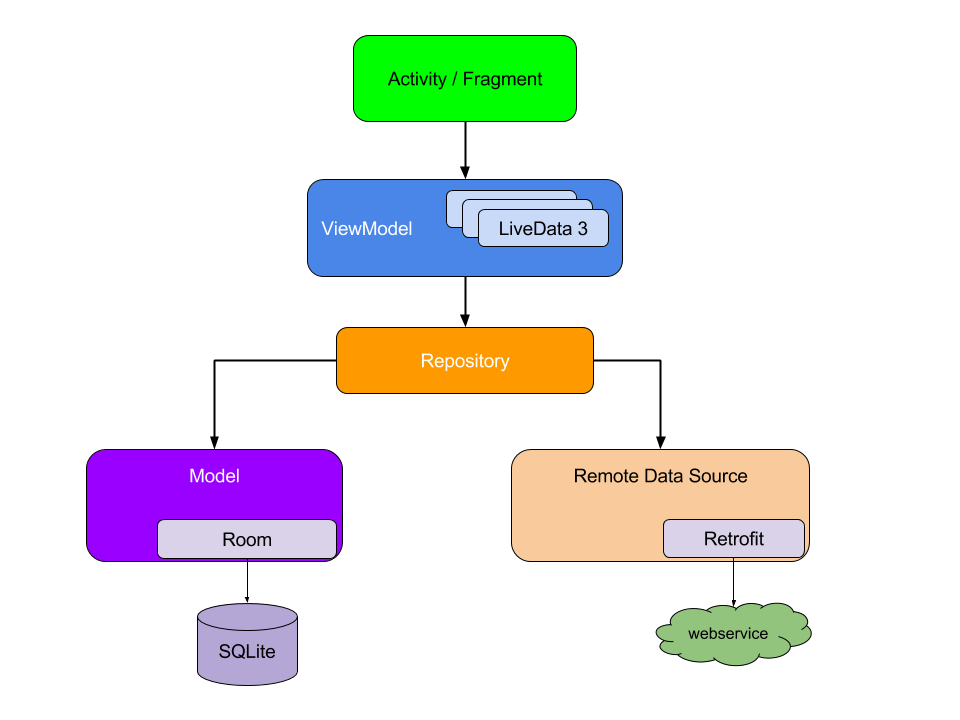
\includegraphics[height=8cm,keepaspectratio]{./images/mvvm-architecture.png}
	\caption{MVVM-Entwurfsmuster \autocite{mvvm_architecture}}
	\label{fig:technologies:architecture:mvvm}
\end{figure}

Benutzeroberflächen, welche in dieser App durch \textit{Fragmente} realisiert wurden, verwenden \textit{Databinding} um von \textit{ViewModels} bereitgestellte Daten anzuzeigen.
Der dafür notwendige Quelltext wird automatisch generiert, wodurch Fehleranfälligkeit reduziert und Entwicklung beschleunigt werden.
Die Verwendung von \textit{LiveData} ermöglicht zudem eine automatische Aktualisierung von Benutzeroberflächen bei Veränderung des Datenbestandes.

\textit{ViewModels} sind für das Verhalten von Benutzeroberflächen verantwortlich und beziehen ihre Daten wiederum aus Datenquellen, welche in Form von \textit{Repositories} implementiert sind.
Einem \textit{ViewModel} ist das besitzende Fragment nicht bekannt, wodurch es unabhängig von Benutzeroberflächen verwendbar ist.

\textit{Repositories} dienen als \textit{Single Point of Truth}, wodurch fehlerhafte oder inkonsistente Datenbestände vermieden werden.
Sie sind an die interne Datenbank (siehe \autoref{subsubsec:technologies:bibs:room}) sowie verschiedene Netzwerkquellen (siehe \autoref{subsec:technologies:apis}) angebunden.


\subsection{APIs}
\label{subsec:technologies:apis}
Um eine Simulation mit echten Kursdaten zu ermöglichen wurden zwei Schnittstellen angebunden.
Sie verwenden unterschiedliche Datenstrukturen, weshalb separate Modelle implementiert wurden.
Die API-spezifischen Antworten der Schnittstellen werden jedoch zu einem einheitlichen Datenmodell transformiert, so dass das Domänenmodell der App simpel und leichtgewichtig bleibt.
Beide APIs erfordern Zuschreibungen, welche im Settings-Screen vorhanden sind (siehe \autoref{subsec:functionality:settings}).


\subsubsection{CoinGecko}
\label{subsubsec:technologies:apis:coingecko}
% https://www.coingecko.com/
\textit{CoinGecko}\footnote{Siehe \url{https://www.coingecko.com/}} stellt Informationen über Kryptowährungen bereit.
Dazu zählen Symbol, Name und Wechselkurse.
Bei letzteren wird nur auf den USD Wechselkurs zurückgegriffen.
Darüber hinaus sind Marktdiagrammdaten verfügbar, die für Kursgraphen verwendet werden.


\subsubsection{IEX Cloud}
\label{subsubsec:technologies:apis:iex}
% https://iexcloud.io/
\textit{IEX Cloud}\footnote{Siehe \url{https://iexcloud.io/}} stellt allgemeine Finanzdaten zur Verfügung.
Nicht alle Daten sind kostenlos zugänglich, weshalb nur Aktieninformationen über diese Schnittstelle bezogen werden.
Analog zu \textit{CoinGecko} liefert \textit{IEX Cloud} Symbole, Namen, aktuelle Preise und Marktdiagrammdaten zu Aktien.
Des Weiteren besitzt \textit{IEX Cloud} Informationen über kurzfristige Änderungen von Aktienkursen und bietet Sammlungen von Neuigkeiten zu einzelnen Aktien.


\subsection{Bibliotheken}
\label{subsec:technologies:bibs}
Im Laufe der Entwicklung wurden verschiedene Bibliotheken von Drittherstellern verwendet, um den notwendigen Programmierungsaufwand zu reduzieren.
Im Folgenden werden diese näher vorgestellt und ihre Vorzüge sowie Eigenschaften erläutert.


\subsubsection{Android Jetpack}
\label{subsubsec:technologies:bibs:jetpack}
Android Jetpack ist eine Sammlung von Bibliotheken, Programmen und Anleitungen. Ziel ist es, das Entwickeln von qualitativ hochwertigen Applikationen zu vereinfachen. Dies wird erreicht, indem dem Entwickler Elemente vorgegeben werden, wodurch weniger Boilerplate-Code geschreiben werden muss und komplizierte Prozesse stark vereinfacht werden \cite{android_jetpack}. Zu erkennen ist die Verwendung einer Jetpack Library an dem Namespace \textit{androidx.*}. Die Libraries sind unabhängig von der Platform API verwendbar. Dadurch wird Abwärtskompatibilität gewährleistet und der Entwickler bekommt plattformunabhängige und häufigere Updates der Libraries. Die Android Jetpack Komponenten lassen sich in vier Anwendungsgebiete, \textit{Fundation}, \textit{Architecture}, \textit{Behavior} und \textit{UI} einteilen. \textit{Fundation} Komponenten stellen beispielweise die Abwärtskompatibilität sicher, beinhalten ein Testframework und Ermöglichen das Arbeiten mit der Programmiersprache Kotlin. \textit{Architecture} Komponenten unterstützen den Programmierer, robusten, testbaren und wartbaren Quellcode zu schreiben. Beispielkomonenten für diesen Abwendungsbereich sind \textit{LiveData}, \textit{Data Binding}, \textit{Room} und der \textit{WorkManager}. \textit{Behavior} Komponenten ermöglichen den einfacheren Umgang mit Android Services, wie Benachrichtigungen, Kamera und Berechtigungen. \textit{UI} Komponenten erleichtern die Entwicklung der Benutzeroberfläche, beispielsweise durch \textit{Fragments}.

Zusätzlich zu den Libraries, welche in diesem Abschnitt erläutert werden, wurden weitere Libraries aus Android Jetpack verwendet, die im Folgenden vorgestellt werden.

\textit{Android KTX} erweitert die Sprache Kotlin um zusätzliche Funktionen. Diese sind hilfreich, um Kotlin unkompliziert in Kombination mit Android, Jetpack und anderen APIs nutzen zu können \autocite{android_ktx}.

\textit{Appcompat} \autocite{android_appcompat} ermöglicht die Nutzung der \textit{Action Bar} \autocite{android_action_bar} in der Benutzeroberfläche. Außerdem unterstützt diese Library das nachträgliche Hinzufügen von dem \textit{material design} System, welches in \autoref{subsubsec:technologies:bibs:material} beschrieben wurde.

\textit{Fragments} stellen ein Verhalten oder einen Teil der Benutzeroberfläche dar \autocite{android_fragments}. Eine \textit{Activity} ist modular aus mehreren \textit{Fragments} aufgebaut und ermöglicht es zur Laufzeit \textit{Fragments} hinzuzufügen oder zu entfernen.

\textit{Layouts} definieren die Anordnung der Benutzeroberfläche bzw. der \textit{Activities} \autocite{android_layouts}. Die Struktur wird hierarchisch aus allen Elementen aufgebaut, die dem Benutzer angezeigt werden sollen. Um die sichtbaren Elemente zu positionieren, können sogenannte, unsichtbare \textit{ViewGroup} Elemente zu Hilfe genommen werden. Verwendet wurden in dieser Applikation die \textit{ViewGroups} \textit{ConstraintLayout} \autocite{android_constraintlayout} und \textit{SwipeRefreshLayout} \autocite{android_swiperefreshlayout}. \textit{ConstraintLayouts} ermöglichen die Positionierung und Größenanpassung der Elemente in flexibler Weise. \textit{SwipeRefreshLayouts} werden immer dort verwendet, wo der Benutzer den Inhalt der Ansicht durch eine vertikale Wischgeste aktualisieren kann.


\subsubsection{Room}
\label{subsubsec:technologies:bibs:room}
% https://developer.android.com/jetpack/androidx/releases/room
Die Room-Persistenzbibliothek stellt eine Abstraktionsschicht über SQLite \footnote{Siehe \url{https://de.wikipedia.org/wiki/SQLite}} dar. Ihr Ziel ist es, Datenbankanfragen zu vereinfachen und "die volle Leistung von SQLite zu nutzen" \cite{android_room_architecture}. Die Bibliothek hilft dabei, einen Cache der Anwendungsdaten auf dem Gerät zu erstellen. Dieser fungiert als Single Source of Truth und stellt sicher, dass eine konsistente Kopie der Anwendungsinformationen zur Verfügung steht. Durch die lokale Speicherung der Daten kann der Nutzer, auch offline auf diese Inhalte zugreifen. Alle Inhaltsänderungen, die vom Benutzer vorgenommen werden, werden mit dem Server synchronisiert, sobald das Gerät wieder online ist.\newline
Room besteht im Wesentlichen aus drei Komponenten: \textit{Database}, \textit{Entity} und \textit{Dao}. \textit{Database} enthält den Datenbankinhaber und fungiert als Hauptzugriffspunkt für die Verbindung zu den persistenten Daten der Anwendung. \textit{Entity} entspricht einer Datenbanktabelle. \textit{Dao} beinhaltet die Methoden für den Zugriff auf die Datenbank. Die Anwendung nutzt die Room-Datenbank um an die Data-Access-Objects (DAOs) zu gelangen. Anschließend werden die einzelnen DAOs verwendet, um die Entitäten aus der Datenbank abzurufen und Änderungen in die Datenbank zu schreiben. Die Entitäten werden dazu verwendet, um die entsprechenden Werte der Datenbanktabellen abzurufen und zu schreiben \cite{android_room_data_storage}. Das Beziehung zwischen drei Komponenten wird in Abbildung \ref{fig:room} dargestellt.

\begin{figure}[H]
	\centering
	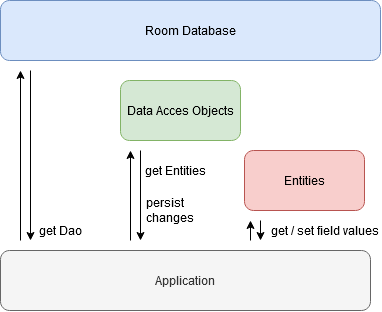
\includegraphics[height=7cm,keepaspectratio]{./images/Room.png}
	\caption{Room Architektur}
	\label{fig:room}
\end{figure}


\subsubsection{WorkManager}
\label{subsubsec:technologies:bibs:workmanager}
% https://developer.android.com/jetpack/androidx/releases/work
% https://developer.android.com/topic/libraries/architecture/workmanager
WorkManager ist eine in Android Jetpack enthaltene Bibliothek \autocite{android_workmanager}. Sie vereinfacht das Ausführen von Hintergrundaufgaben, sogenannten Workern. Es existieren zwei verschiedene Arten, einmalige und periodische Worker. Mithilfe des WorkManagers werden die Worker besonders ressourcensparend, vorallem aber energiesparend im Hintergrund ausgeführt. \textit{Constraints} ermöglichen es, Bedingungen an den Worker zu knüpfen, beispielweise das Benötigen einer Internetverbindung. Mittels \textit{Data} werden dem Worker Daten übergeben, welche gegebenenfalls für die Ausführung benötigt werden. Einmalige Worker eignen sich besonders für Aufgaben, die zurückgestellt werden können und nicht im Vordergrund zu Erledigen sind. Periodische Worker können immer dort eingesetzt werden, wo mit den gleichen Einstellungen regelmäßig Arbeit verrichtet werden soll. Das kleinstmögliche Intervall ist bei periodischen Workern auf 15 Minuten beschränkt.


\subsubsection{Moshi}
\label{subsubsec:technologies:bibs:moshi}
% https://github.com/square/moshi
TODO


\subsubsection{Retrofit}
\label{subsubsec:technologies:bibs:retrofit}
% https://github.com/square/retrofit
TODO


\subsubsection{MPAndroidChart}
\label{subsubsec:technologies:bibs:mpandroidchart}
% https://github.com/PhilJay/MPAndroidChart
\textit{MPAndroidChart} \autocite{mpandroidchart} ermöglicht die Darstellung von Diagrammen unter Android. Unterstützt werden alle gängigen Diagrammtypen, sowie Kombinationen von mehreren Typen in einem Diagramm. Durch die vielen Konfigurationsmöglichkeiten können die Diagramme passgenau auf das Anwendungsgebiet abgestimmt werden. In dieser Applikation wurden mithilfe der Library der Verlauf des Kontostands, des Depots und des Aktienkurses visualisiert.


\subsubsection{Biometric-Auth}
\label{subsubsec:technologies:bibs:biometricauth}
% https://github.com/anitaa1990/Biometric-Auth-Sample
TODO


\subsubsection{Picasso}
\label{subsubsec:technologies:bibs:picasso}
% https://github.com/square/picasso
\textit{Picasso} \autocite{picasso} ist eine Library, die das Herunterladen und Zwischenspeichern von Bildern ermöglicht. Durch die Zwischenspeicherung wird zum Einen Datenvolumen gespart und zum Anderen die Performance der Benutzeroberfläche bei mehrmaligen Aufrufen erhöht. In der Applikation wurde die Library für die Anzeige von News verwendet, welche mit Bildern ausgeliefert werden (siehe \autoref{subsec:functionality:news}).


\subsubsection{Material}
\label{subsubsec:technologies:bibs:material}
% https://material.io/develop/android/docs/getting-started/
\textit{Material} ist ein Designsystem, welches unter anderem von Google entwickelt wird.
Mit UI-Elementen der offiziellen \textit{Material}-Bibliothek war es möglich moderne Benutzeroberflächen zu erstellen, ohne Entwicklungszeit für Design und Implementierung dieser zu verwenden
\textit{Material} wurde für das App-Theme sowie die \textit{Bottom Navigation} (siehe \autoref{subsec:functionality:navigation}) verwendet.


\subsubsection{Timber}
\label{subsubsec:technologies:bibs:timber}
% https://github.com/JakeWharton/timber
\textit{Timber} ist eine Schnittstelle, welche auf der Android \textit{Log}-Klasse aufbaut und das Loggen von Ereignissen vereinfacht.
Dadurch war es möglich Entwicklungszeit zu sparen und Programmierfehler schnell ausfindig zu machen.
Durch Verwendung von \textit{Timber} werden Log-Nachrichten zudem nur während der Entwicklung, und nicht in der fertigen App, ausgegeben.


\subsubsection{Dokka}
\label{subsubsec:technologies:bibs:dokka}
% https://github.com/Kotlin/dokka
\textit{Dokka} ist eine "`documentation engine"' und wird zum Generieren von Quelltextdokumentationen verwendet.
Es handelt sich also nicht um eine Bibliothek, die in der App verwendet wird, sondern um ein Entwicklungswerkzeug.
Mit \textit{Dokka}  wird die Dokumentation des Quelltextes dieser App generiert\footnote{Siehe \url{https://deryeger.github.io/stock-simulator/app/}}.


\section{Funktionalität}
\label{sec:functionality}
% Welche Features habt ihr gebaut?
% Welche Screens habt ihr gebaut?
% Warum sehen die Screens so aus? (warum ist button X an Position Y) / was habt ihr euch dabei gedacht?
Im Folgenden wird die Funktionalität der App, nach Screens aufgeteilt, vorgestellt.


\subsection{Navigation}
\label{subsec:functionality:navigation}
Über die \textit{Bottom Navigation} \autocite{bottom_navigation} können Nutzer zwischen den Hauptfeatures Account, Suche, Transaktionsverlauf, Stockbrot und Errungenschaften wechseln (siehe \autoref{fig:functionality:navigation:screens}).
Diese Art der Navigation wurde gewählt, da sie modernen Designempfehlungen entspricht und bessere Kompatibilität mit Android 10 Gesten aufweist als beispielsweise ein \textit{Hamburger Menü}.

Das Einstellungsmenü ist über das Zahnrad in der Toolbar aller Screens, au"ser den Einstellungen selbst, erreichbar (siehe \autoref{fig:functionality:navigation:screens}).

Weitere Navigation, wie zu den News oder zur Detailansicht eines Anlageguts, ist über Bedienelemente in Form von Buttons an entsprechenden Stellen möglich.

\autoref{fig:functionality:navigation:screens} stellt den Navigationsgraph zwischen den einzelnen Bildschirmen dar.
\begin{figure}[H]
	\centering
	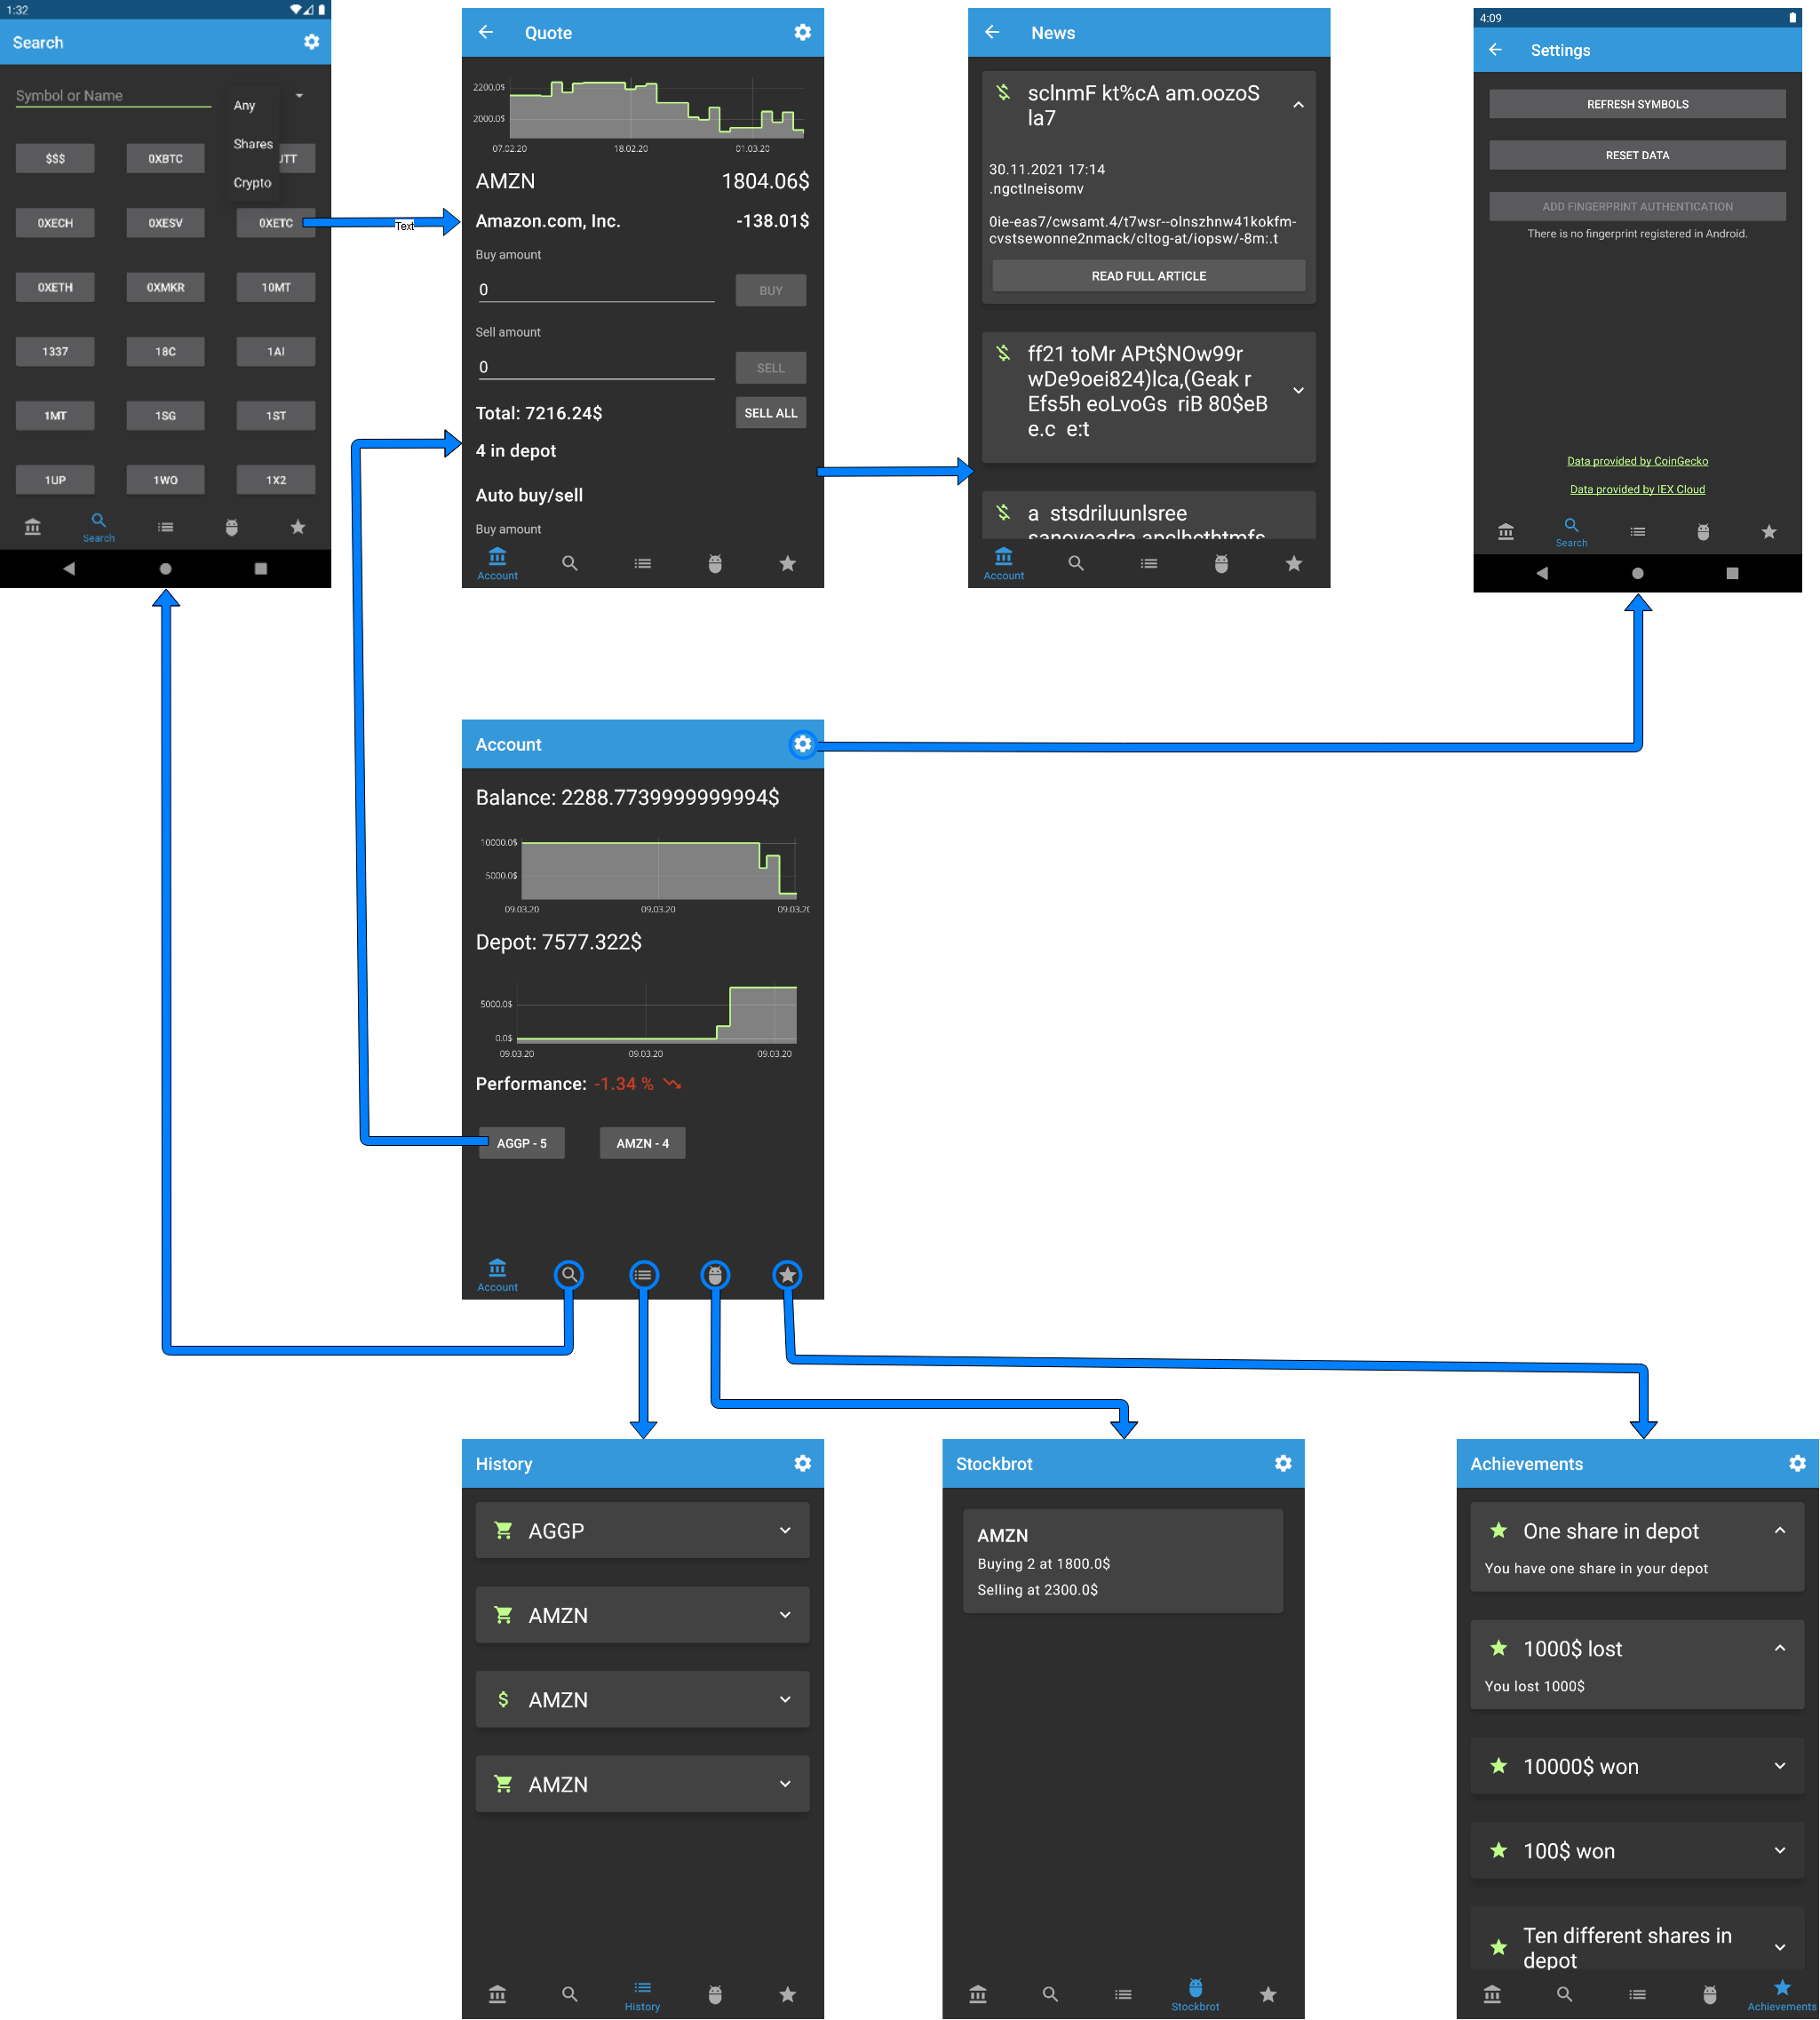
\includegraphics[height=12cm]{./images/navigation_screens/navigation_screens.png}
	\caption{Navigation zwischen den Bildschirmen}
	\label{fig:functionality:navigation:screens}
\end{figure}


\subsection{Account}
\label{subsec:functionality:account}
TODO


\subsection{Suche}
\label{subsec:functionality:search}
Das Suchen von Aktien und Kryptowährungen nach Name und Symbol ist im Search-Screen möglich.
Zudem können Nutzer dort auswählen, ob sie nur Aktien oder Kryptowährungen sehen möchten.

Das Eingabefeld für Suchanfragen und die Dropdown-Liste zum Filtern befinden sich am oberen Bildschirmrand (siehe \autoref{fig:functionality:search:full}).
Darunter werden Suchergebnisse in einem scrollbaren Raster angezeigt (siehe \autoref{fig:functionality:search:results}).
Diese Aktualisieren sich automatisch, sobald sich ein Suchkriterium verändert.
Dadurch ist es möglich auf Nutzereingaben unmittelbar zu reagieren und Ergebnisse schnell anzuzeigen.
Während eine Suche stattfindet wird ein Fortschritts\-indikator angezeigt, um Nutzer über den aktuellen Zustand zu informieren (siehe \autoref{fig:functionality:search:loading}).
Sollte eine Suche keine Ergebnisse liefern wird eine entsprechende Meldung angezeigt (siehe \autoref{fig:functionality:search:no-results}).

Durch Klicken auf ein Suchergebnis können Nutzer zur Detailansicht dieses Anlageguts navigieren (siehe \autoref{subsec:functionality:quote}).

\begin{figure}[H]
	\begin{subfigure}{.5\textwidth}
		\centering
		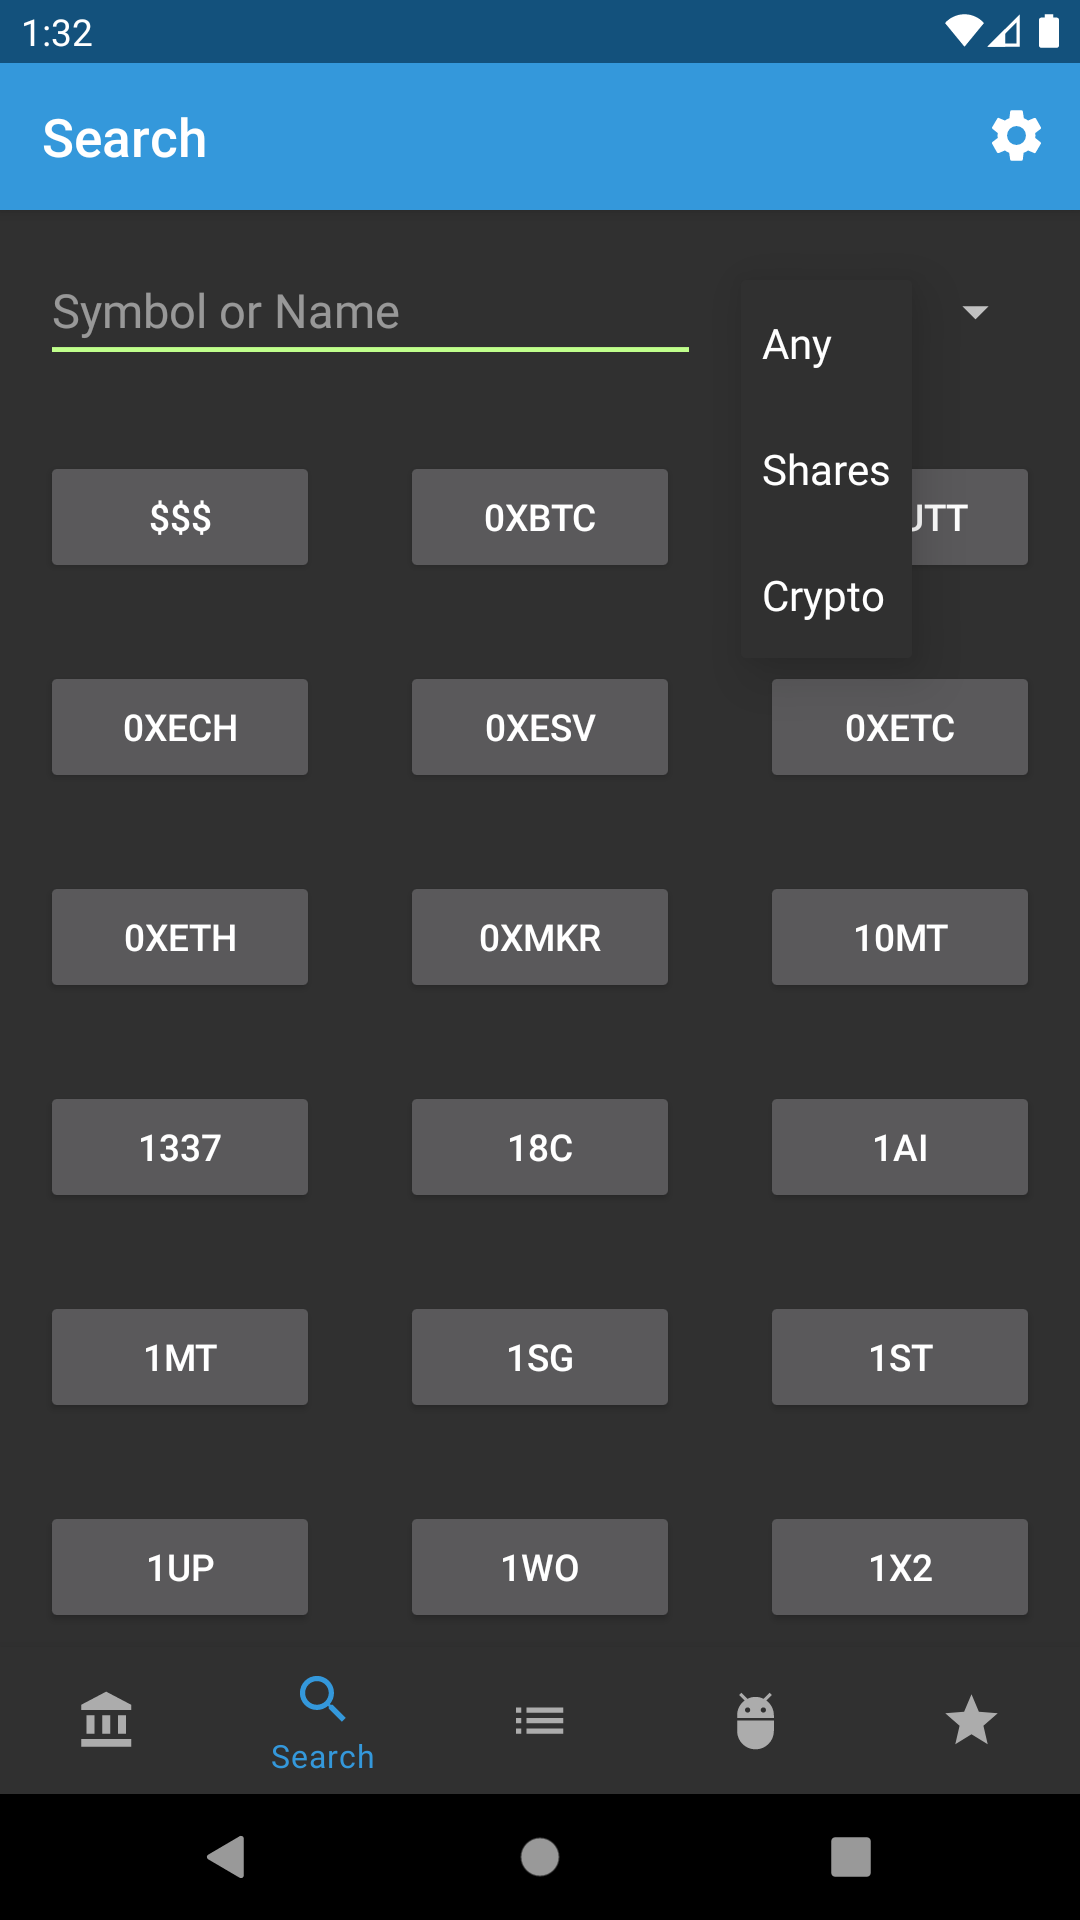
\includegraphics[height=8cm,keepaspectratio]{./images/search/type.png}
		\caption{Nutzereingabe}
		\label{fig:functionality:search:full}
	\end{subfigure}
	\begin{subfigure}{.5\textwidth}
		\centering
		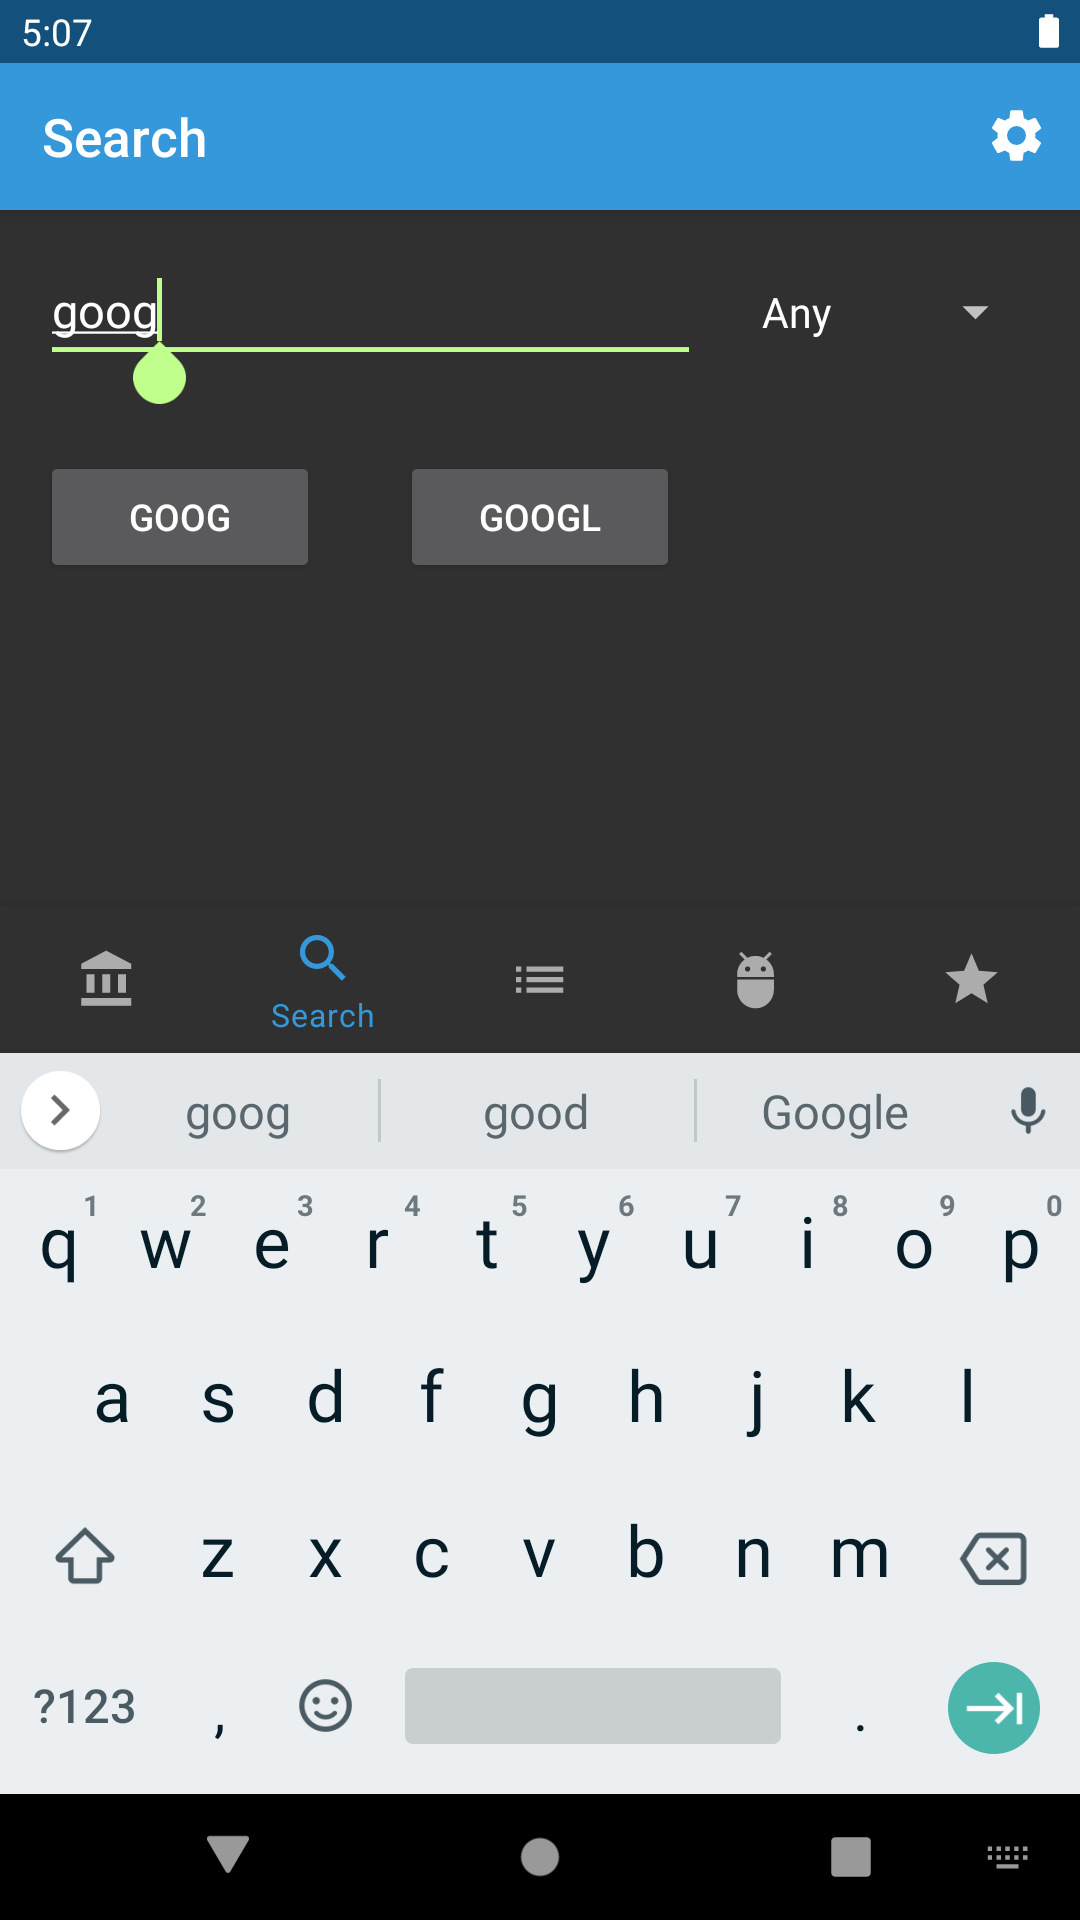
\includegraphics[height=8cm,keepaspectratio]{./images/search/done.png}
		\caption{Suchergebnisse}
		\label{fig:functionality:search:results}
	\end{subfigure}
	\begin{subfigure}{.5\textwidth}
		\centering
		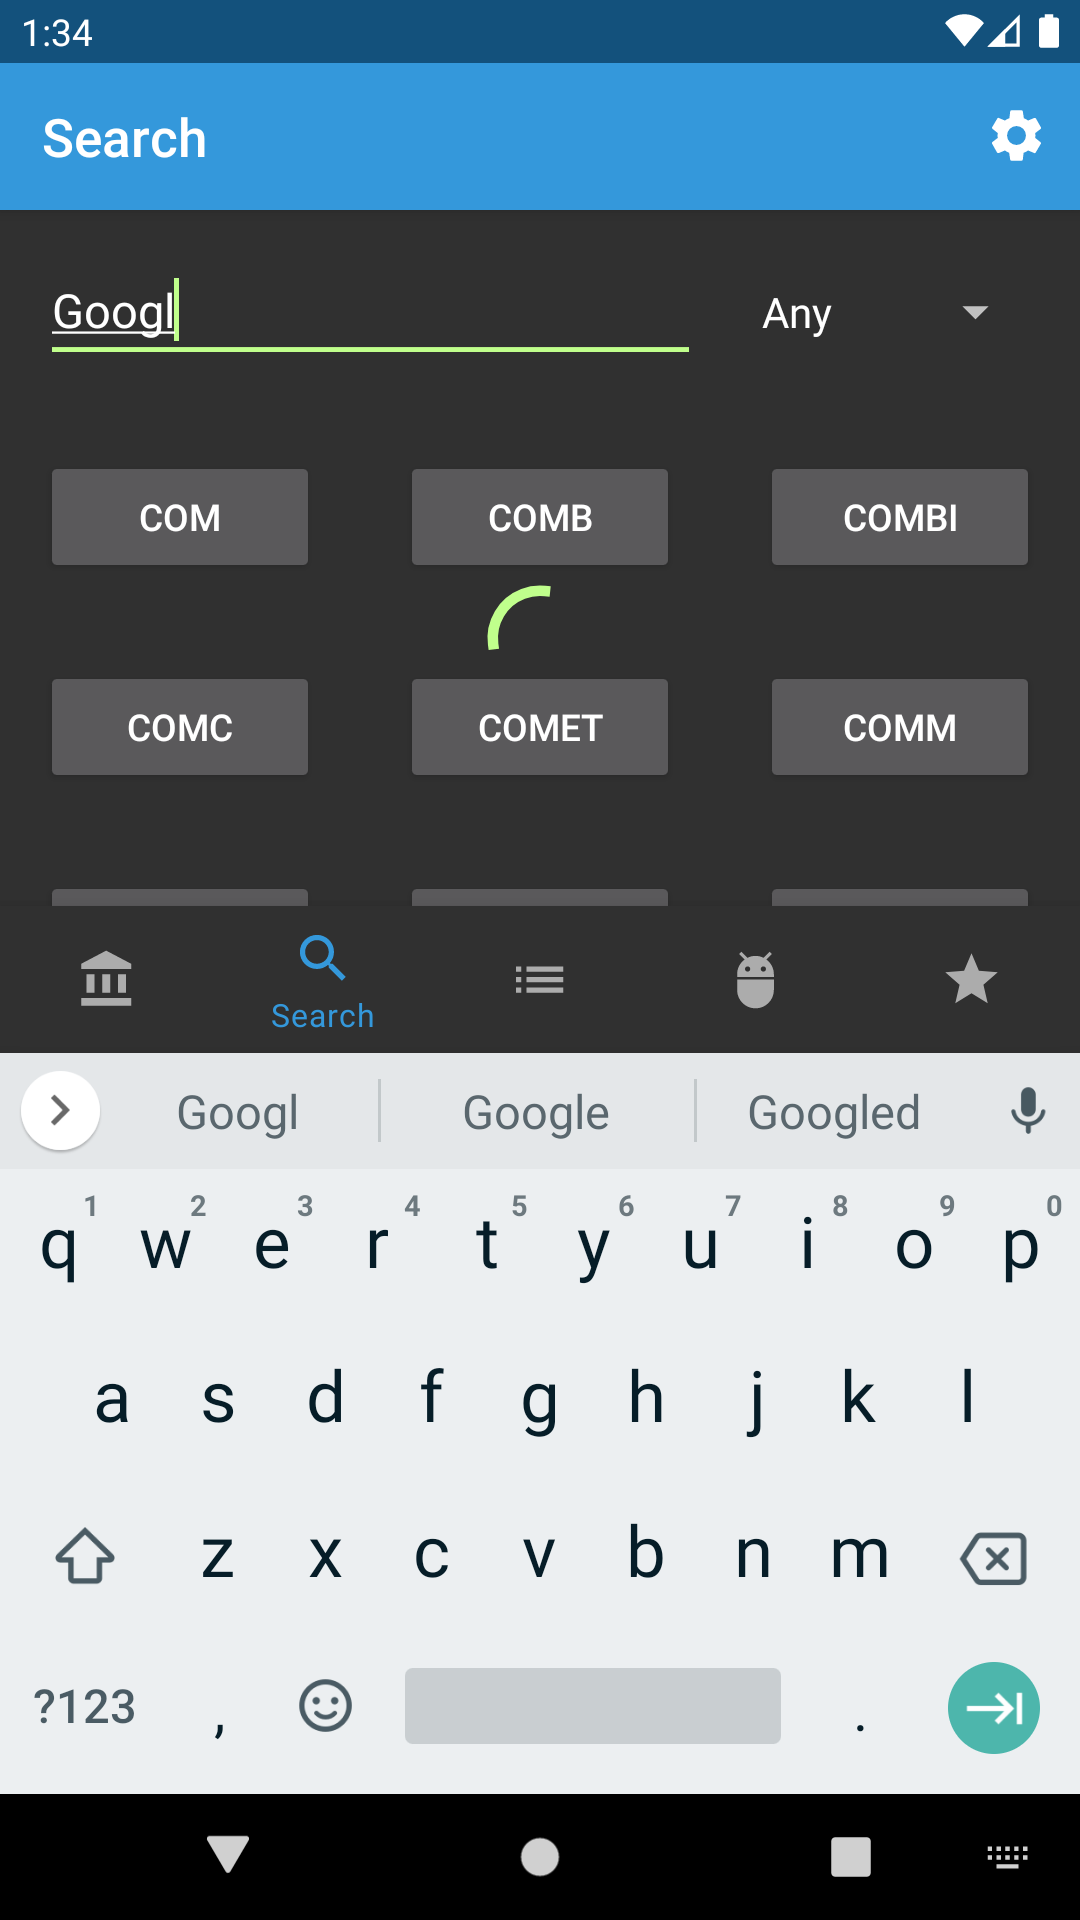
\includegraphics[height=8cm,keepaspectratio]{./images/search/loading.png}
		\caption{Fortschrittsindikator}
		\label{fig:functionality:search:loading}
	\end{subfigure}
	\begin{subfigure}{.5\textwidth}
		\centering
		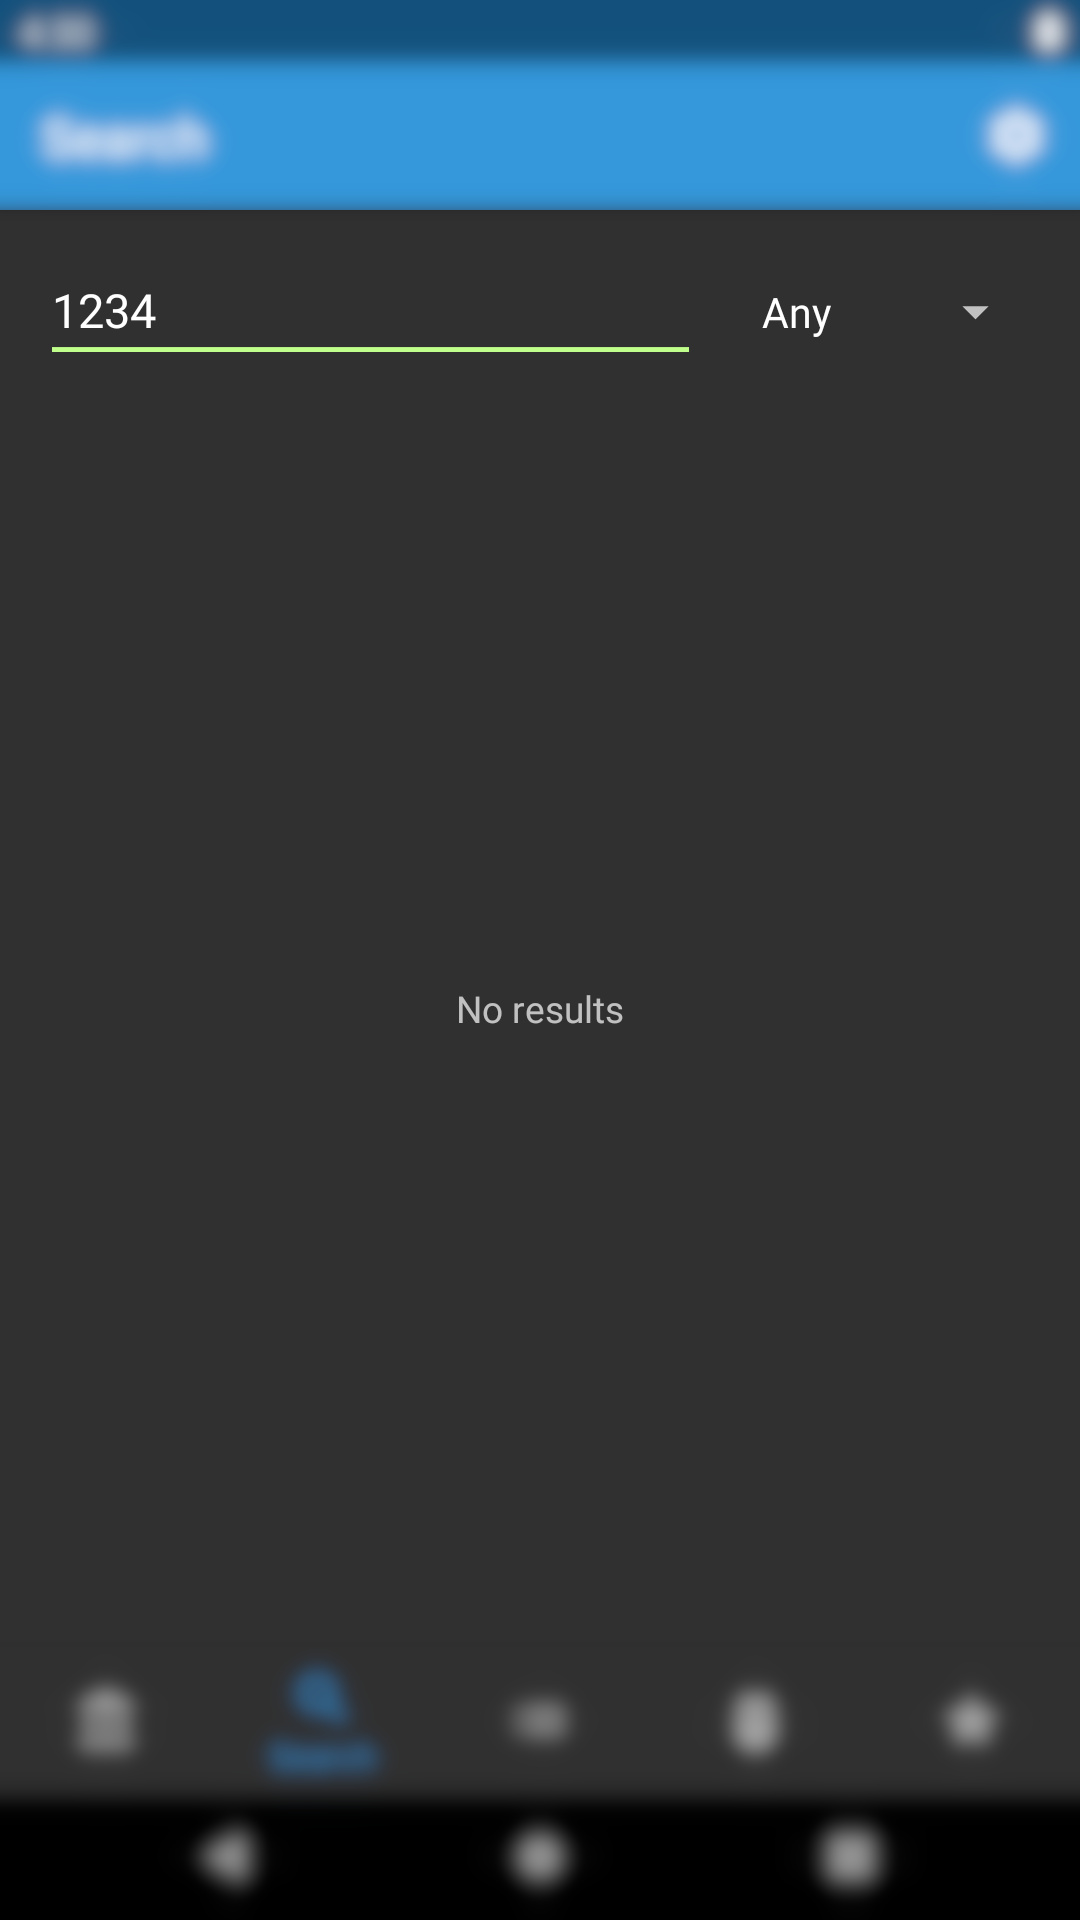
\includegraphics[height=8cm,keepaspectratio]{./images/search/no_results.png}
		\caption{Suche ohne Ergebnisse}
		\label{fig:functionality:search:no-results}
	\end{subfigure}
	\caption{Suche}
	\label{fig:functionality:search}
\end{figure}


\subsection{Transaktionsverlauf}
\label{subsec:functionality:history}
Eine Übersicht über alle getätigten Transaktionen, das heißt Ein- und Verkäufe von Aktien und Cryptocoins, werden im History-Screen dargestellt. Dieser wird über den ''History''-Eintrag der Bottom Navigation erreicht. In \autoref{fig:functionality:history:list} ist der Aufbau des History-Screens zu sehen. Transaktionen werden in Form von ausklappbaren Karten dargestellt.

\begin{figure}[H]
	\centering
	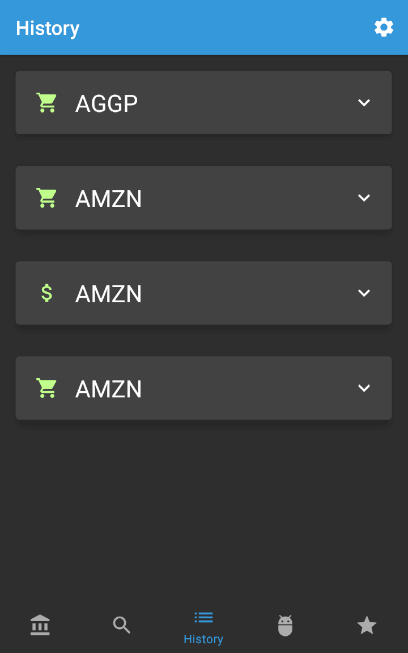
\includegraphics[height=7cm,keepaspectratio]{./images/history_list.png}
	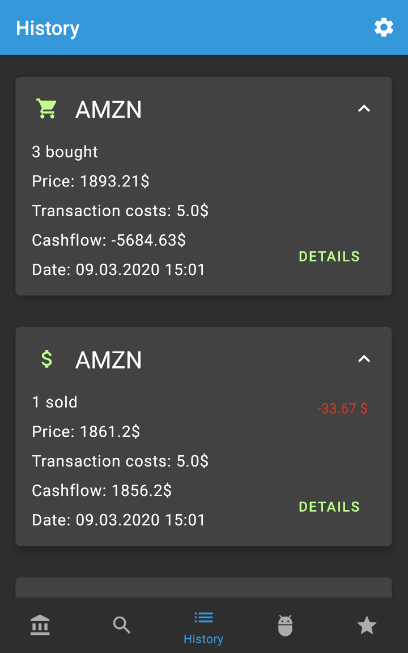
\includegraphics[height=7cm,keepaspectratio]{./images/history_list_open.png}
	\caption{History}
	\label{fig:functionality:history:list}
\end{figure}

Die Karten sind nach dem Zeitpunkt ihrer Durchführung absteigend geordnet, sodass die älteste Transaktion zu Beginn positioniert ist. Eine Karte beinhaltet das Symbol der jeweiligen Anlage und ein Icon, mit dem angezeigt wird, ob es sich bei der Transaktion um einen Kauf (Einkaufswagen) oder einen Verkauf (Dollar-Symbol) handelt. Durch Klick auf den Pfeil kann eine Transaktionskarte ausgeklappt werden, um die Details der jeweiligen Transaktion anzuzeigen. In der Detailansicht wird angezeigt, wie viele Anlagen ge- oder verkauft wurden, der Preis dieser Anlage zum Zeitpunkt der Transaktion, die Transaktionskosten, der dadurch bewirkte Geldfluss (Cashflow) sowie das Datum und die Uhrzeit, zu der die Transaktion durchgeführt wurde. Zusätzlich wird bei einem Verkauf angezeigt, wie hoch der Gewinn bzw. Verlust durch diesen Verkauf war.


\subsection{Stockbrot}
\label{subsec:functionality:stockbrot}
Der Name Stockbrot leitet sich aus den Begriffen stock (deutsch: Aktie) und Bot ab. Mithilfe dieses Bots ist der Benutzer in der Lage das Traden von Aktien oder Kryptowährungen zu automatisieren. Für jede Anlage, welche sich unter der Kontrolle des Bots befindet, wird ein sogenannter Worker alle 15 Minuten ausgeführt. Von dem Worker wird geprüft, ob die zuvor in der Detailansicht (\autoref{subsec:functionality:quote}) festgelegten Schwellwerte des aktuellen Kurses erreicht wurden. Falls dies der Fall ist, wird eine entsprechende Transaktion ausgeführt. Die Worker werden im Hintergrund mithilfe des \textit{WorkManagers} gesteuert.

\autoref{fig:functionality:stockbrot:overview} zeigt den Screen, der eine Übersicht über die von dem Stockbrot verwalteten Aktien und Kryptowährungen liefert. Die Navigation zu diesem Screen erfolgt über einen Klick auf den Eintrag "`Stockbrot"' in der Bottom Navigation. Wenn zuvor keine Aktien oder Kryptowährungen zu dem Bot hinzugefügt wurden, werden in diesem Screen keine Einträge aufgelistet (\autoref{fig:functionality:stockbrot:overview:empty}). Sobald eine Aktie/Kryptowährung der Kontrolle des Bots über die Detailansicht einer Anlage (\autoref{subsec:functionality:quote}) übergeben wurde, wird diese als Element der Liste angezeigt (\autoref{fig:functionality:stockbrot:overview:entry}). Jedes dieser Elemente besteht aus der Id, sowie den Schwellwerten, bei deren Unter- oder Überschreitung der Bot einen Kauf- oder Verkauf veranlassen soll.

\begin{figure}[H]
    \begin{subfigure}{.5\textwidth}
        \centering
        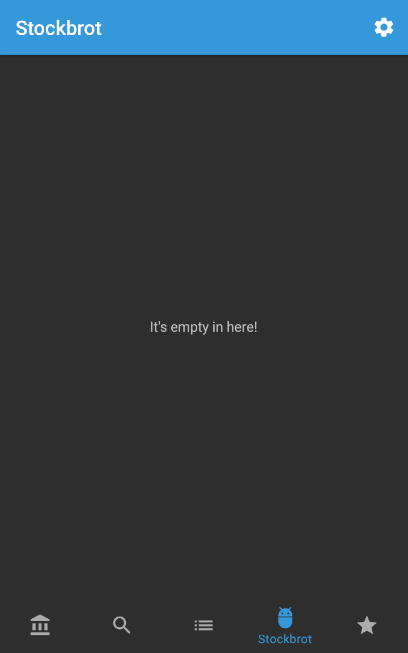
\includegraphics[height=8cm,keepaspectratio]{./images/stockbrot_list_empty.png}  
        \caption{Stockbrot Übersicht ohne Eintrag}
        \label{fig:functionality:stockbrot:overview:empty}
    \end{subfigure}
    \begin{subfigure}{.5\textwidth}
        \centering
        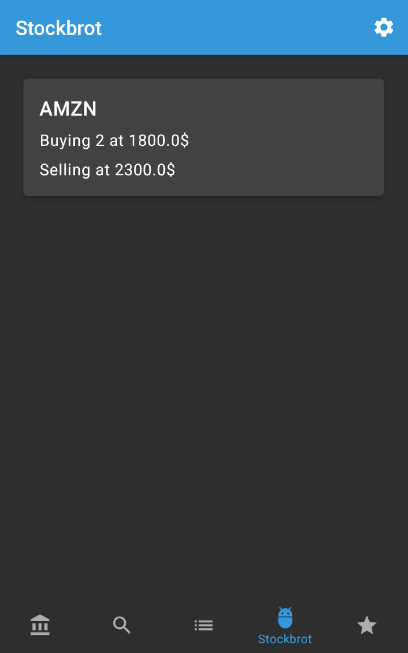
\includegraphics[height=8cm,keepaspectratio]{./images/stockbrot_list.png}  
        \caption{Stockbrot Übersicht mit Eintrag}
        \label{fig:functionality:stockbrot:overview:entry}
    \end{subfigure}
    \caption{Stockbrot Übersicht}
    \label{fig:functionality:stockbrot:overview}
\end{figure}


\subsection{Errungenschaften}
\label{subsec:functionality:achievements}
Um den Benutzer des Spiels vor Herausforderungen zu stellen, sind verschiedene Errungenschaften erreichbar. Eine Übersicht über diese Erfolge, sind in dem Achievements-Screen einsehbar, welcher über den Eintrag "`Achievements"' in der Bottom Navigation zu erreichen ist. Dieser Screen listet, wie in \autoref{fig:functionality:achievements:overview:closed} sichtbar, alle bereits erreichten und noch freizuschaltenden Errungenschaften auf. Die Hintergrundfarben der noch nicht freigeschalteten Errungenschaften, werden in der Liste ausgegraut. Jedes der Elemente besteht aus einem Titel und einer Beschreibung. Die Beschreibung ist für alle bereits erreichten Errungenschaften, mittels Pfeil auf der rechten Seite des Elements, aufklappbar (\autoref{fig:functionality:achievements:overview:open}).

\begin{figure}[H]
    \begin{subfigure}{.5\textwidth}
        \centering
        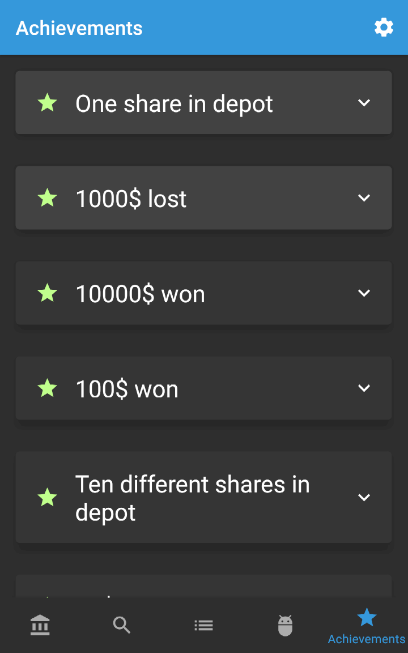
\includegraphics[height=8cm,keepaspectratio]{./images/achievements_list.png}  
        \caption{Errungenschaften Übersicht ohne Beschreibung}
        \label{fig:functionality:achievements:overview:closed}
    \end{subfigure}
    \begin{subfigure}{.5\textwidth}
        \centering
        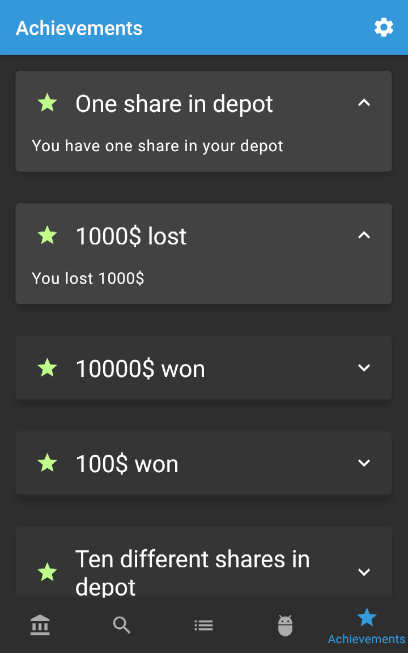
\includegraphics[height=8cm,keepaspectratio]{./images/achievements_list_open.png}  
        \caption{Errungenschaften Übersicht mit Beschreibung}
        \label{fig:functionality:achievements:overview:open}
    \end{subfigure}
    \caption{Errungenschaften Übersicht}
    \label{fig:functionality:achievements:overview}
\end{figure}

Sobald eine Errungenschaft freigeschaltet wird, erscheint im unteren Teil des aktuellen Screens eine Toast-Benachrichtigung \autocite{android_toasts} (siehe \autoref{fig:functionality:achievements:reached}). Diese zeigt den Titel der Errungenschaft an. Beim nächsten Aufruf der Übersicht der Errungenschaften ist dieser soeben erreichte Erfolg nicht mehr ausgegraut und die Beschreibung lässt sich einsehen. Sollten mehrere Errungenschaften direkt hintereinander freigeschaltet werden, werden auch die Benachrichtigungen nacheinander angezeigt. Intern wird sichergestellt, dass kein Erfolgt mehrfach angezeigt wird, selbst wenn die Kriterien zur Freischaltung eines Erfolgs öfter erfüllt werden.

\begin{figure}[H]
    \centering
    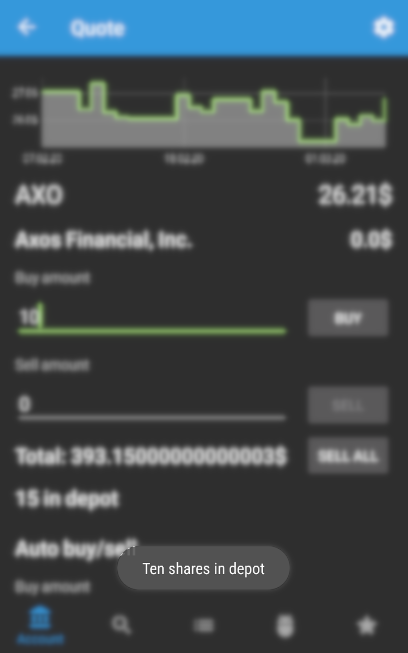
\includegraphics[height=8cm,keepaspectratio]{./images/achievement_reached.png}
    \caption{Errungenschaft wurde erreicht}
    \label{fig:functionality:achievements:reached}
\end{figure}


\subsection{Detailansicht}
\label{subsec:functionality:quote}
In der Detailansicht sind allgemeine Informationen über ein Anlagegut zu sehen (siehe \autoref{fig:functionality:quote:information}).
Dazu zählen Symbol, Name, aktueller Kurs und Kursänderung des Anlageguts.
Sollten keine Informationen über Kursänderungen vorliegen, wird stattdessen "`N/D"' angezeigt.

Darüber wird der Kursverlauf des Anlageguts angezeigt (siehe \autoref{fig:functionality:quote:history}).
Auch hier werden Platzhalter verwendet, falls keine Daten vorliegen sollten.

\begin{figure}[H]
	\begin{subfigure}{.5\textwidth}
		\centering
		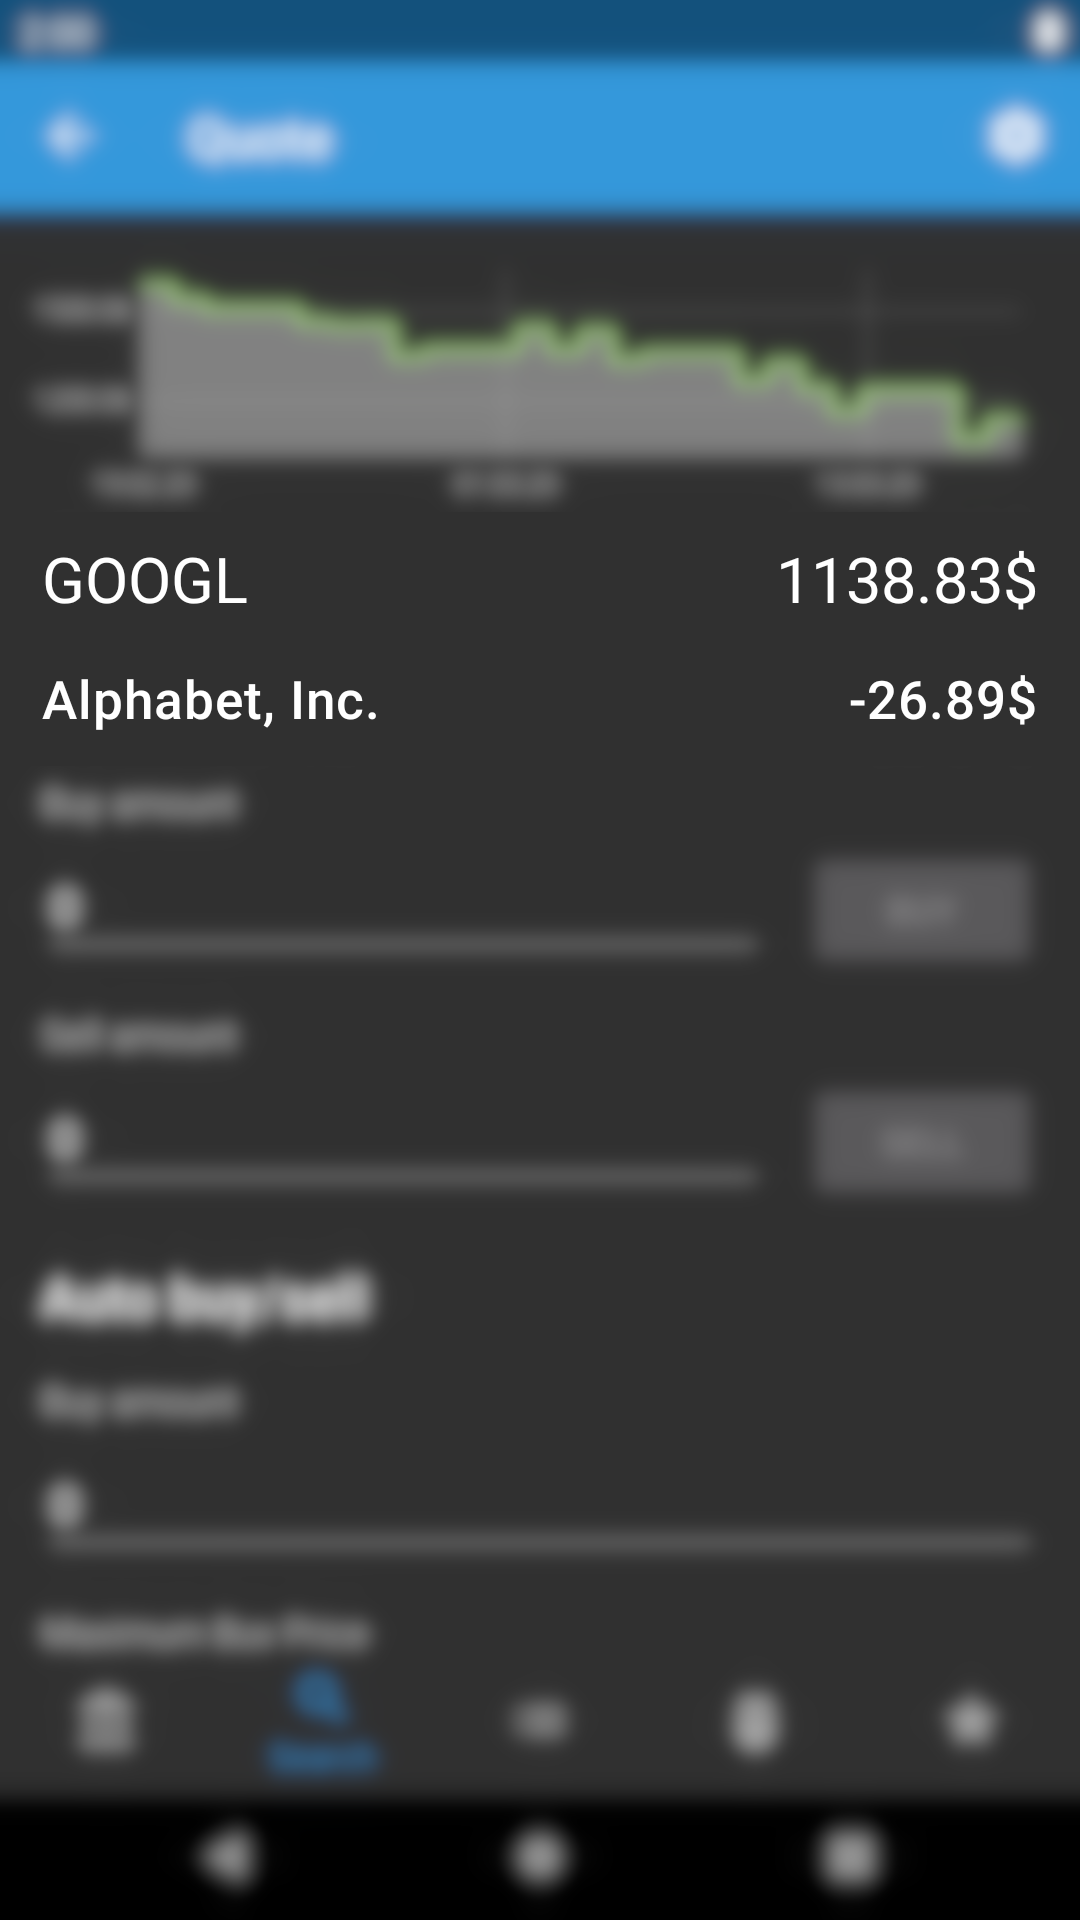
\includegraphics[height=8cm,keepaspectratio]{./images/quote/information.png}
		\caption{Informationen}
		\label{fig:functionality:quote:information}
	\end{subfigure}
	\begin{subfigure}{.5\textwidth}
		\centering
		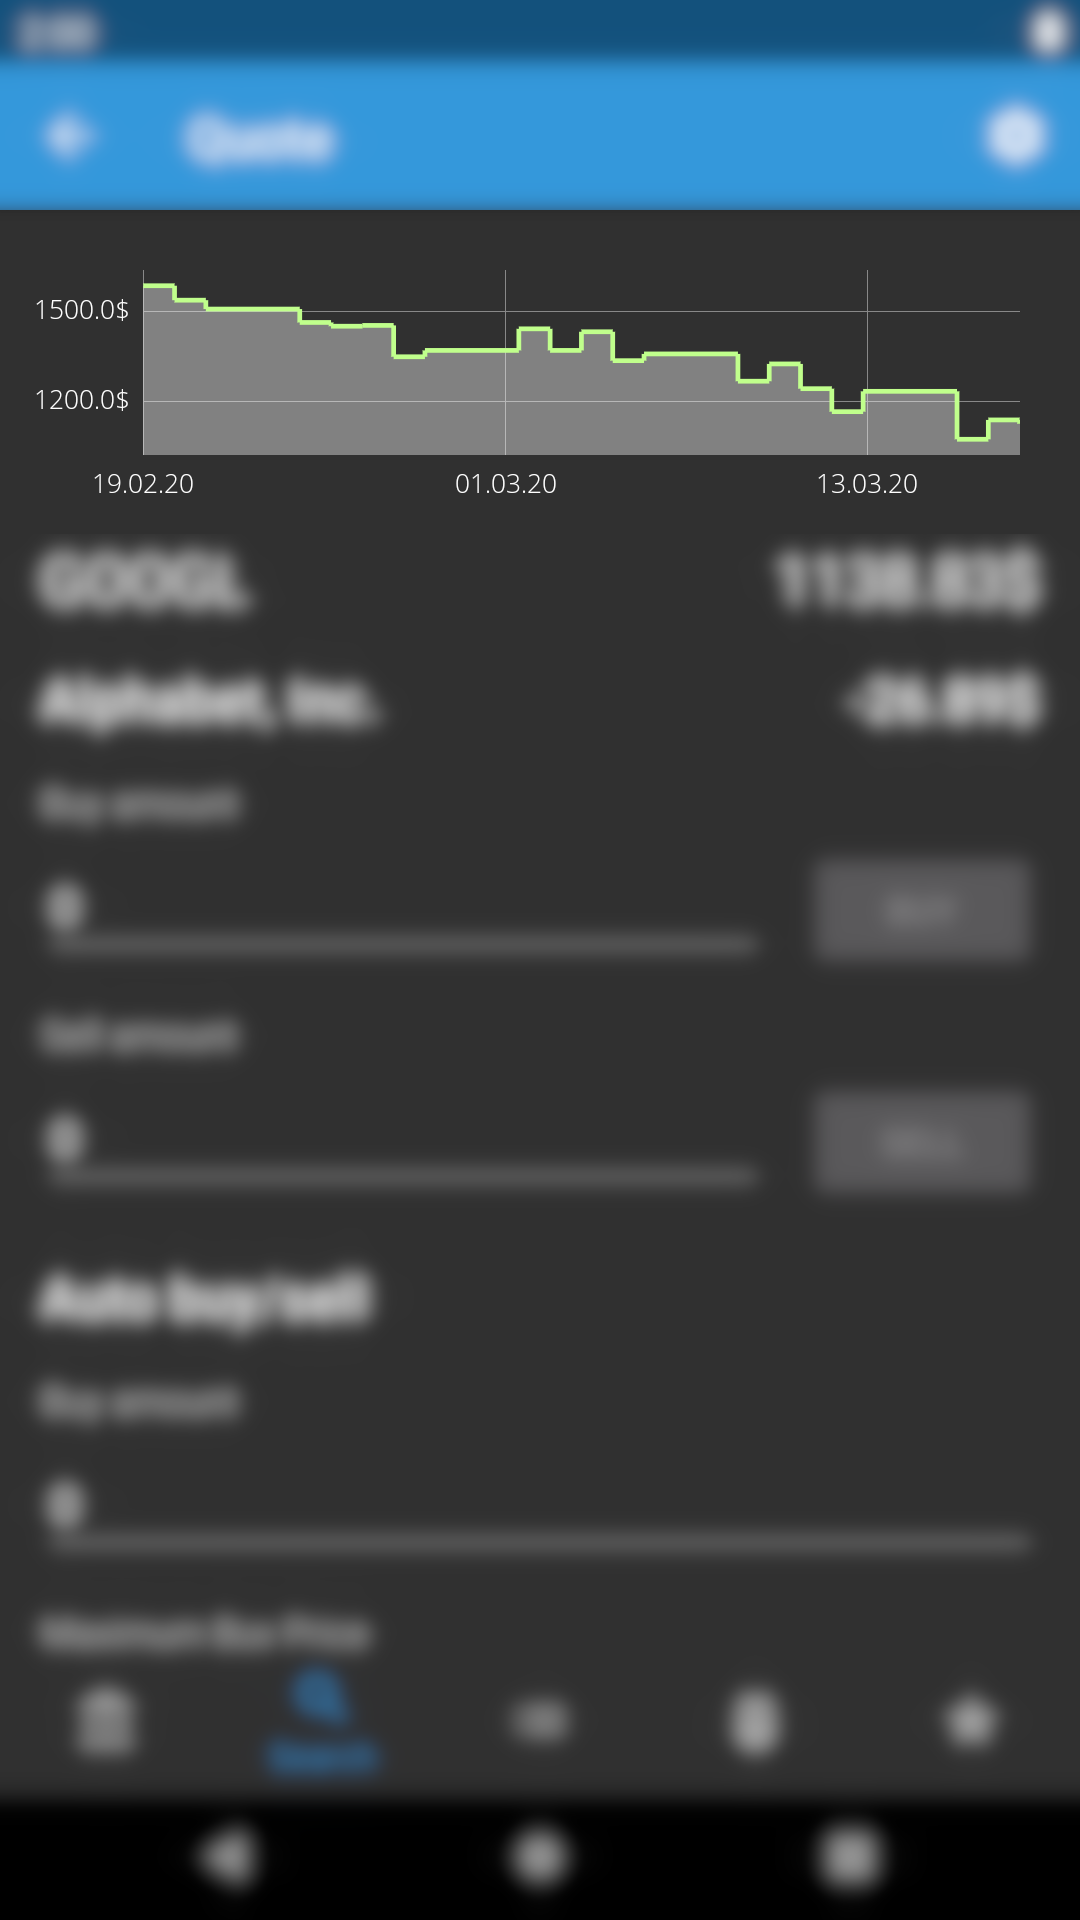
\includegraphics[height=8cm,keepaspectratio]{./images/quote/history.png}
		\caption{Kursverlauf}
		\label{fig:functionality:quote:history}
	\end{subfigure}
	\caption{Detailansicht}
	\label{fig:functionality:quote}
\end{figure}

Kaufen und Verkaufen findet über separate Eingabefelder statt (siehe \autoref{fig:functionality:buy-sell:input}).
Die zugehörigen Buttons sind nur aktiviert, wenn die Eingabe einen Kauf beziehungsweise Verkauf zulässt.

Nach Betätigen eines Buttons müssen Nutzer die Transaktion noch einmal bestätigen.
Der in \autoref{fig:functionality:buy-sell:dialog} dargestellte Bestätigungsdialog zeigt zudem die Transaktionsinformationen erneut an.

Haben Nutzer ein Anlagegut im Depot wird dies ebenfalls in der Detailansicht vermerkt (siehe \autoref{fig:functionality:buy-sell:in-depot}).
Es werden sowohl die Menge als auch der Gesamtwert angezeigt.
Zusätzlich wird der Button "`SELL ALL"' aktiviert, welcher einen Ausverkauf des entsprechenden Anlageguts aus dem Depot durchführt.

\begin{figure}[H]
	\begin{subfigure}{.5\textwidth}
		\centering
		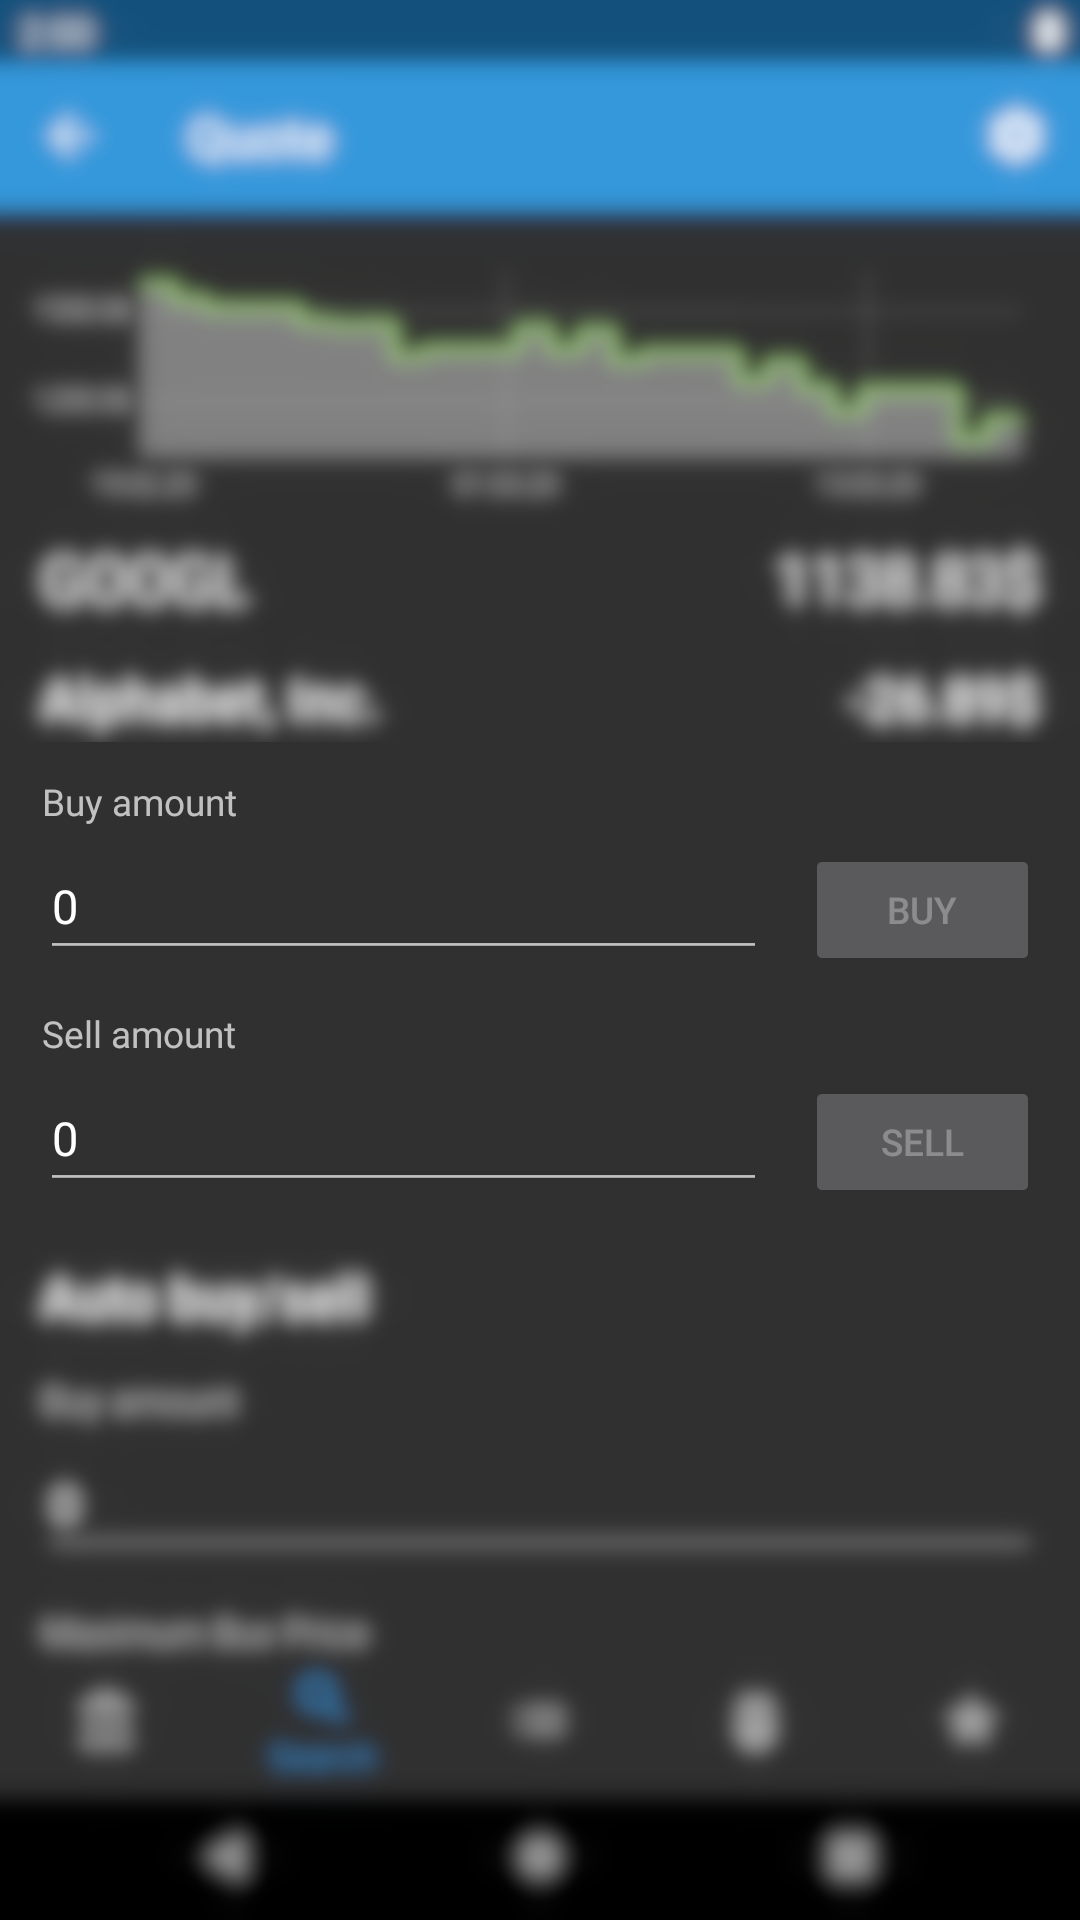
\includegraphics[height=8cm,keepaspectratio]{./images/quote/buy_sell.png}
		\caption{Nutzereingabe}
		\label{fig:functionality:buy-sell:input}
	\end{subfigure}
	\begin{subfigure}{.5\textwidth}
		\centering
		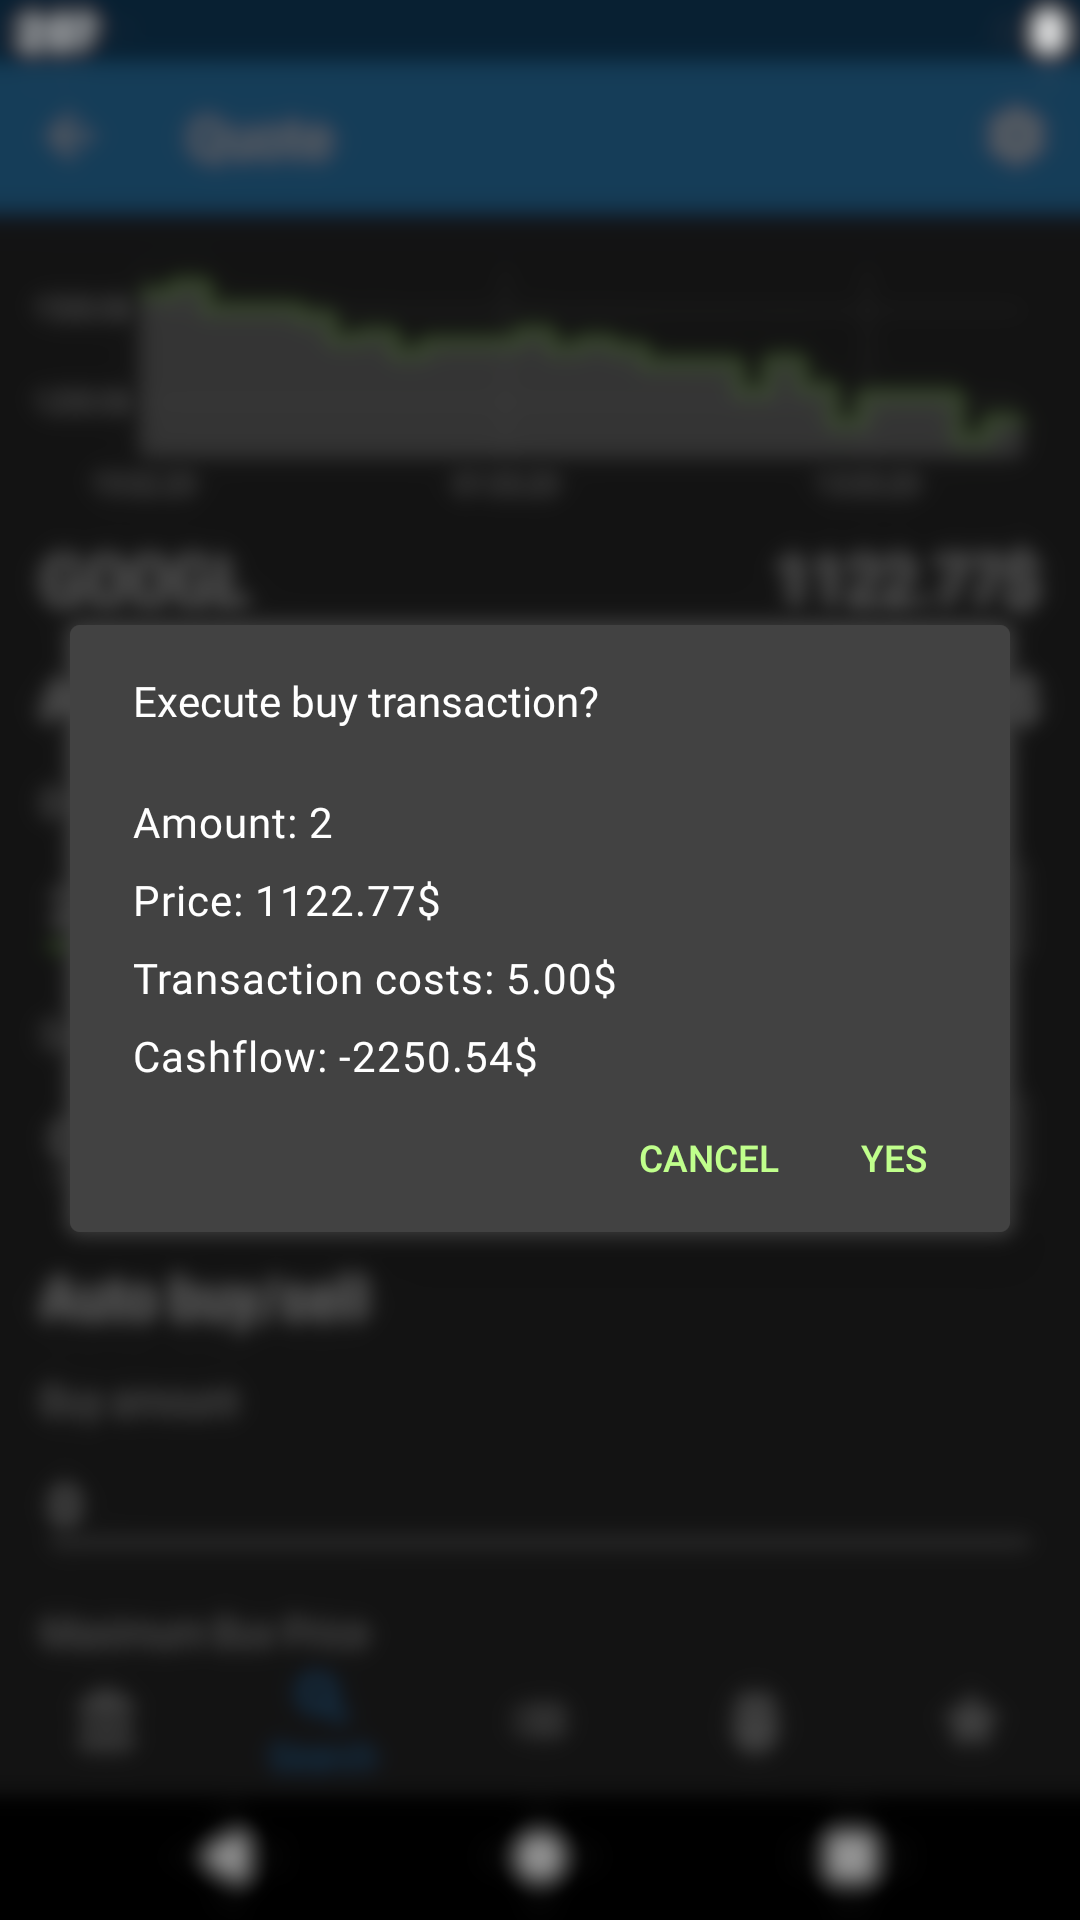
\includegraphics[height=8cm,keepaspectratio]{./images/quote/buy_dialog.png}
		\caption{Bestätigungsdialog}
		\label{fig:functionality:buy-sell:dialog}
	\end{subfigure}
	\begin{subfigure}{.5\textwidth}
		\centering
		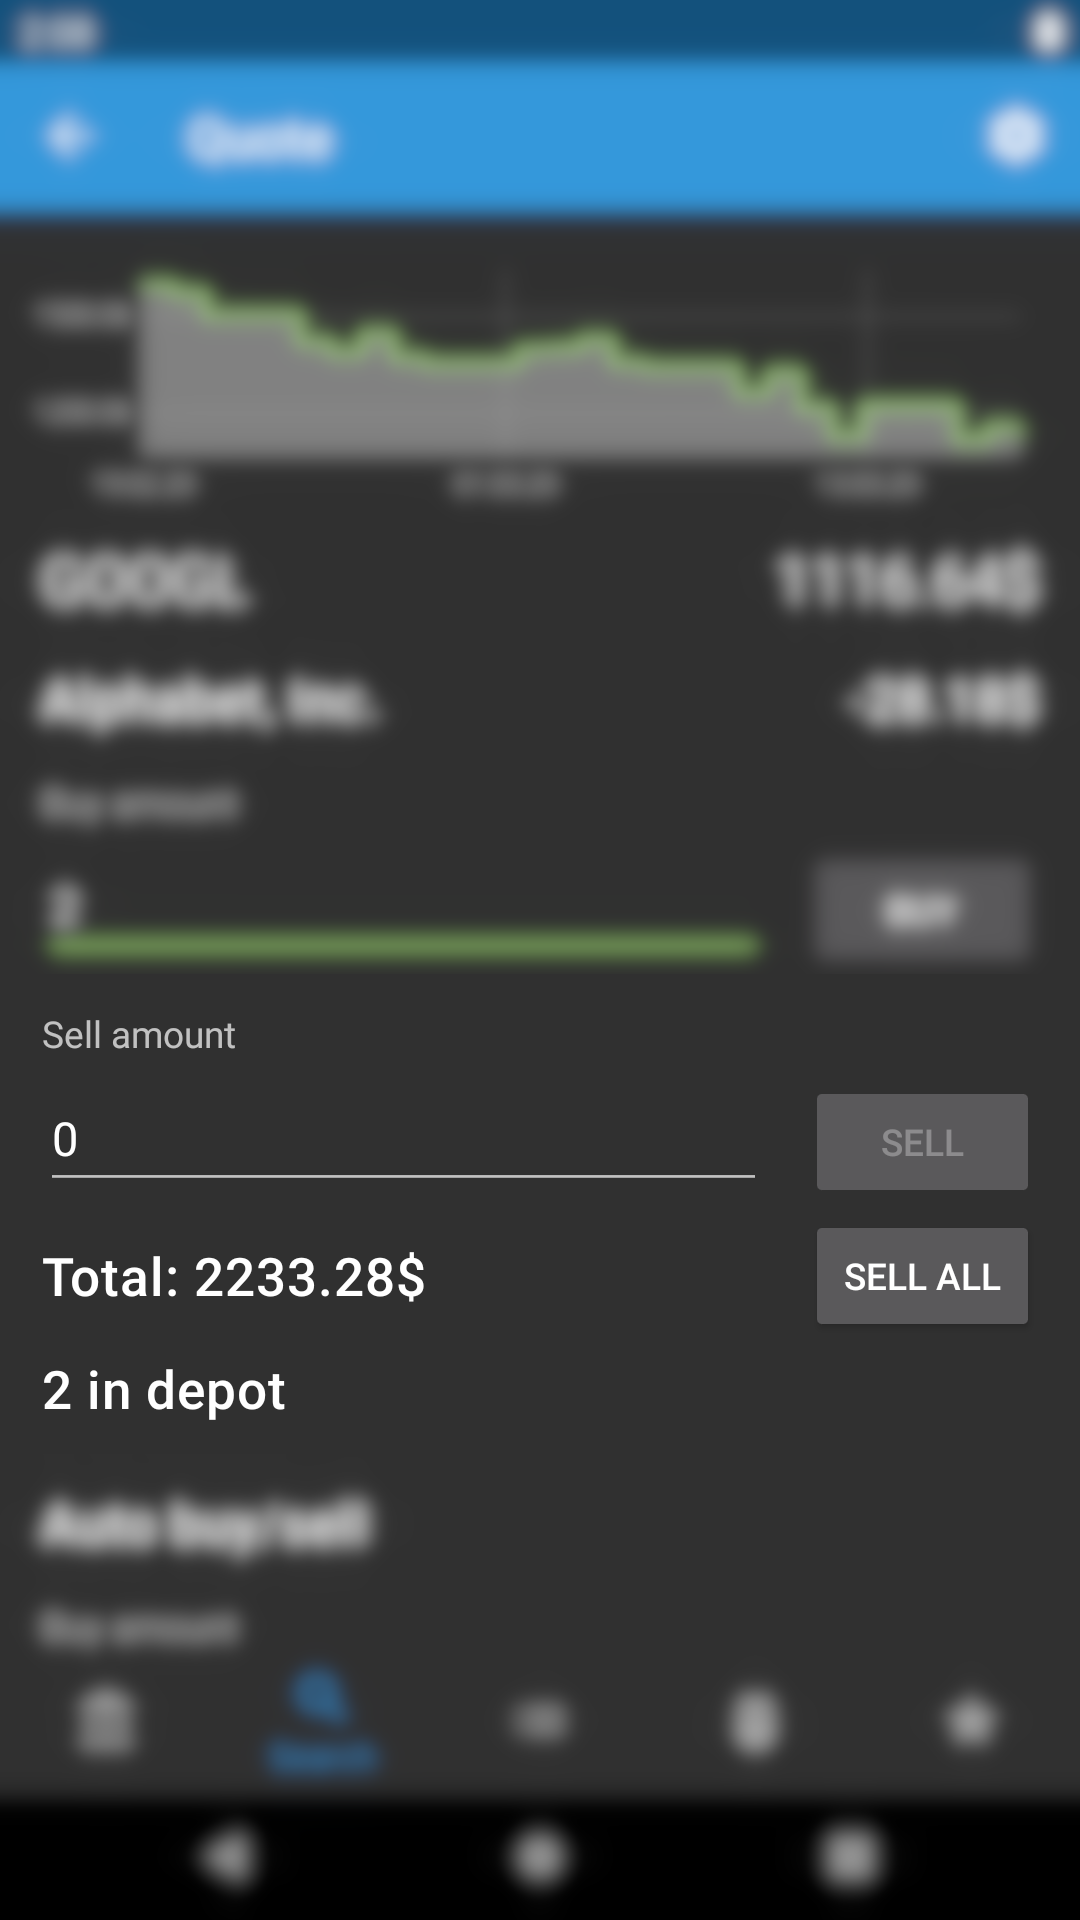
\includegraphics[height=8cm,keepaspectratio]{./images/quote/in_depot.png}
		\caption{Anlage im Depot}
		\label{fig:functionality:buy-sell:in-depot}
	\end{subfigure}
	\caption{Kaufen und Verkaufen}
	\label{fig:functionality:buy-sell}
\end{figure}

\autoref{fig:functionality:stockbrot:addremove} zeigt einen Abschnitt aus der Detailansicht, welcher das Hinzufügen einer Anlage zu dem Bot (\autoref{fig:functionality:stockbrot:add}), sowie das Entfernen dieser (\autoref{fig:functionality:stockbrot:remove}), ermöglicht. In dem Abschnitt, beginnend mit dem Label "`Auto buy/sell"', können Kauf- und Verkaufsoptionen für den Bot festgelegt werden. Ohne Spezifikation der Kaufoptionen, wird die Anlage nicht vom Bot gekauft und ohne Spezifikation der Verkaufsoption, nicht verkauft. Wenn weder Kauf- noch Verkaufsoptionen korrekt spezifiziert wurden, bleibt der Button "`ADD TO STOCKBROT"' ausgegraut. Das Kaufverhalten des Bots kann mittels Textfeld "`Buy amount"' und "`Maximum Buy Price"' festgelegt werden. Mit diesen Optionen wird die maximale Anzahl der zu kaufenden Aktien oder Kryptowährungen, sowie der Schwellwert des Preises festgelegt, unter dem ein Kauf stattfinden soll. Mittels der Textfelder "`Minimum Sell Price"' kann festgelegt werden, welche Grenze der Preis der Anlage überschreiten muss, damit der Bot einen Verkauf durchführt. Wird eine Aktie oder Kryptowährung bereits von dem Bot kontrolliert, kann diese mittels Klick auf den Button "`REMOVE QUOTE FROM STOCKBROT"' wieder der Kontrolle des Bots entzogen werden.

\begin{figure}[H]
    \begin{subfigure}{.5\textwidth}
        \centering
        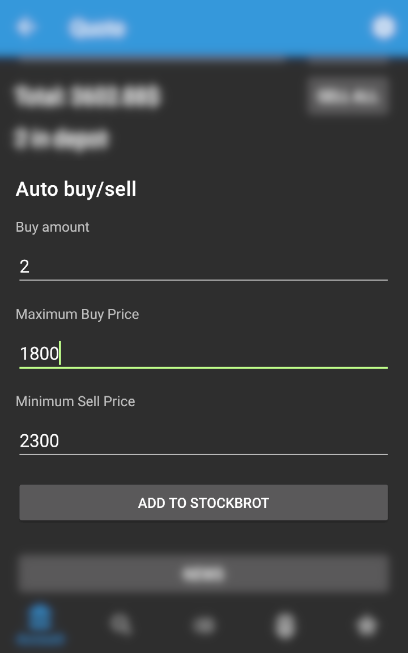
\includegraphics[height=8cm,keepaspectratio]{./images/stockbrot_add_before.png}
        \caption{Anlage zum Stockbrot hinzufügen}
        \label{fig:functionality:stockbrot:add}
    \end{subfigure}
    \begin{subfigure}{.5\textwidth}
        \centering
        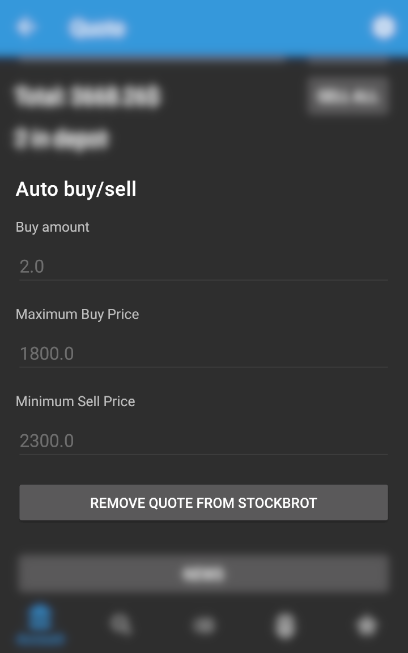
\includegraphics[height=8cm,keepaspectratio]{./images/stockbrot_add_after.png}
        \caption{Anlage vom Stockbrot entfernen}
        \label{fig:functionality:stockbrot:remove}
    \end{subfigure}
    \caption{Anlage zum/vom Stockbrot hinzufügen/entfernen}
    \label{fig:functionality:stockbrot:addremove}
\end{figure}


\subsection{News}
\label{subsec:functionality:news}
TODO


\subsection{Einstellungen}
\label{subsec:functionality:settings}
Der \textit{Settings-Screen} beinhaltet Optionen zum Zurücksetzen von Spieldaten, Aktualisieren der verfügbaren Anlagegüter sowie Hinzufügen und Entfernen einer Fingerabdruck-Sperre.
Wie in \autoref{fig:functionality:settings:buttons} zu sehen sind Buttons der zuvor beschriebenen Optionen vertikal angeordnet.
Der Button zum Hinzufügen und Entfernen einer Fingerabdruck-Sperre ist zudem deaktiviert, falls dies nicht möglich ist.
Ein Informationstext unter diesem Button wei"st Nutzer auf den Zustand hin.

Am unteren Ende des Screens (siehe \autoref{fig:functionality:settings:attributions}) befinden sich die notwendigen Zuschreibungen an die verwendeten Schnittstellen (siehe \autoref{subsec:technologies:apis}).
Durch Klicken auf einen der Links werden Nutzer zur Website der jeweiligen Schnittstelle weitergeleitet.

%TODO Snackbars "demonstrieren"

\begin{figure}[H]
	\begin{subfigure}{.5\textwidth}
		\centering
		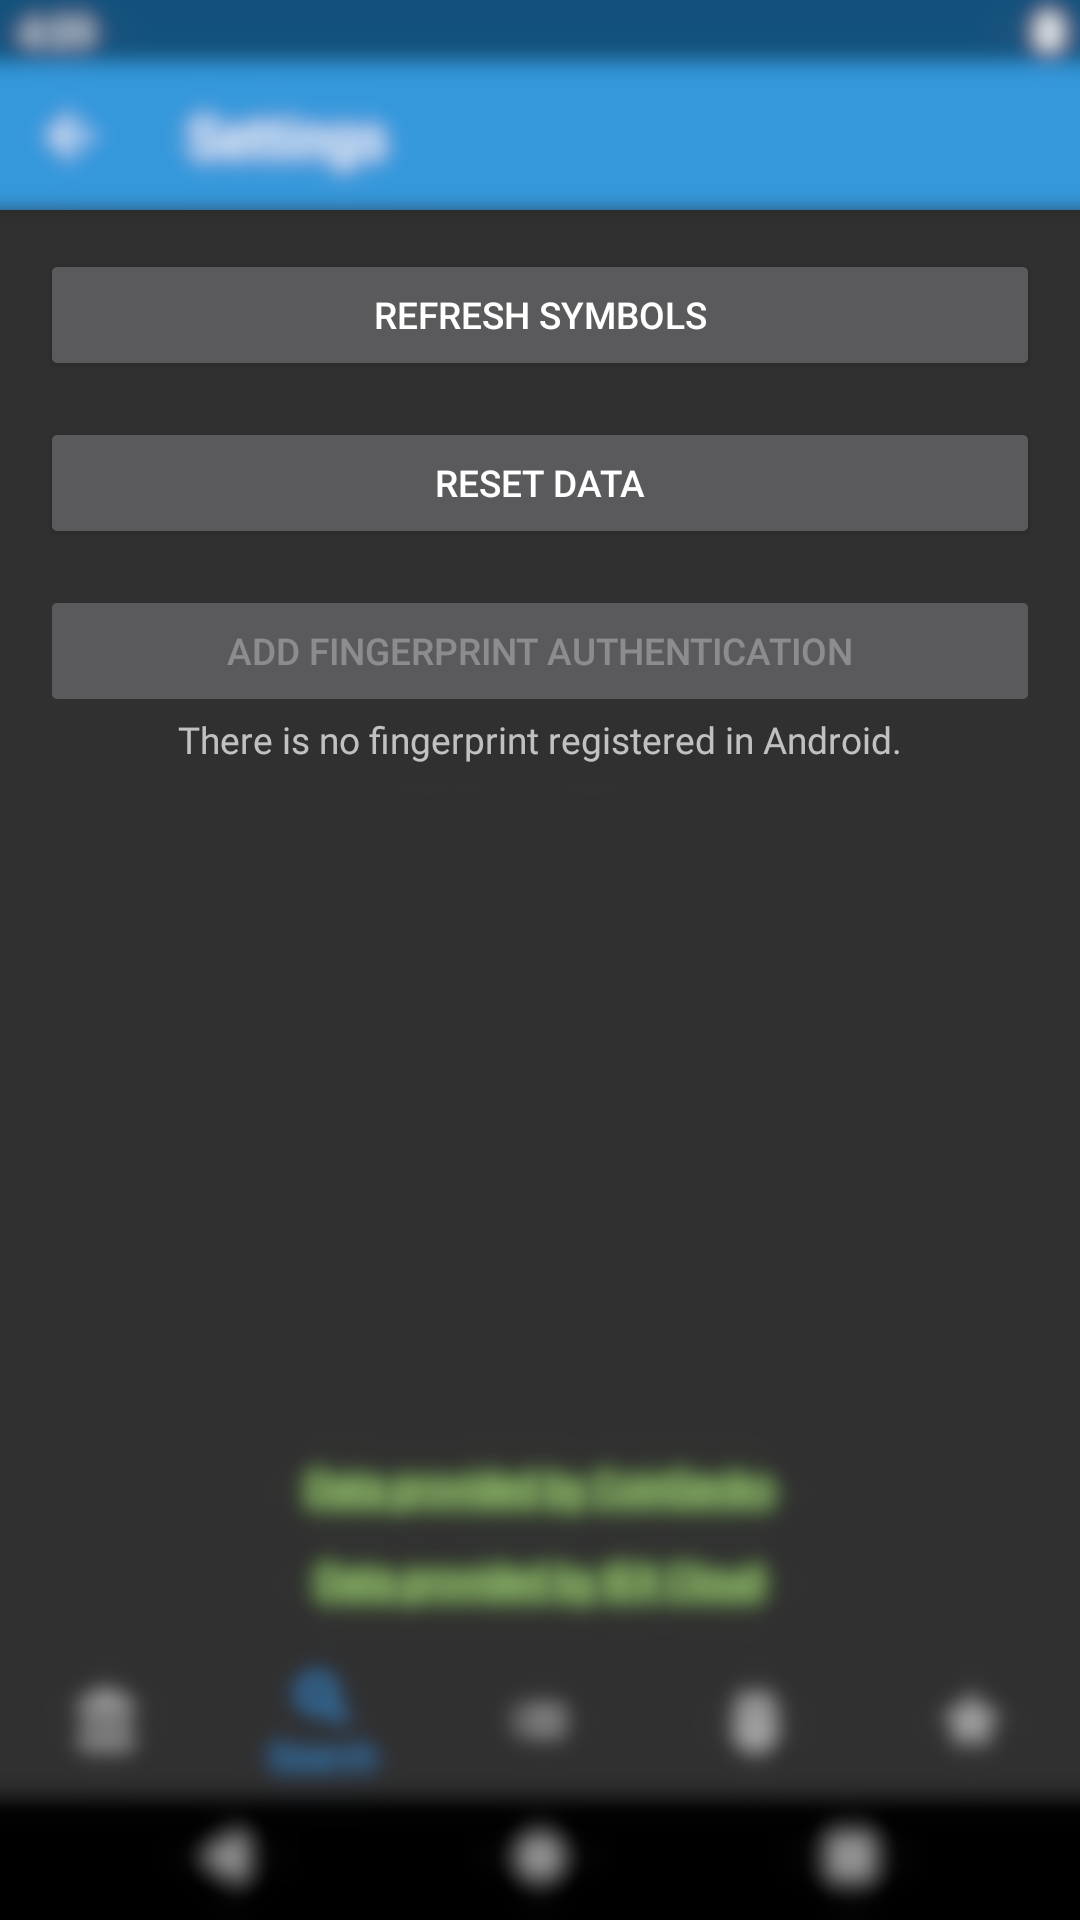
\includegraphics[height=8cm,keepaspectratio]{./images/settings/buttons.png}
		\caption{Optionen}
		\label{fig:functionality:settings:buttons}
	\end{subfigure}
	\begin{subfigure}{.5\textwidth}
		\centering
		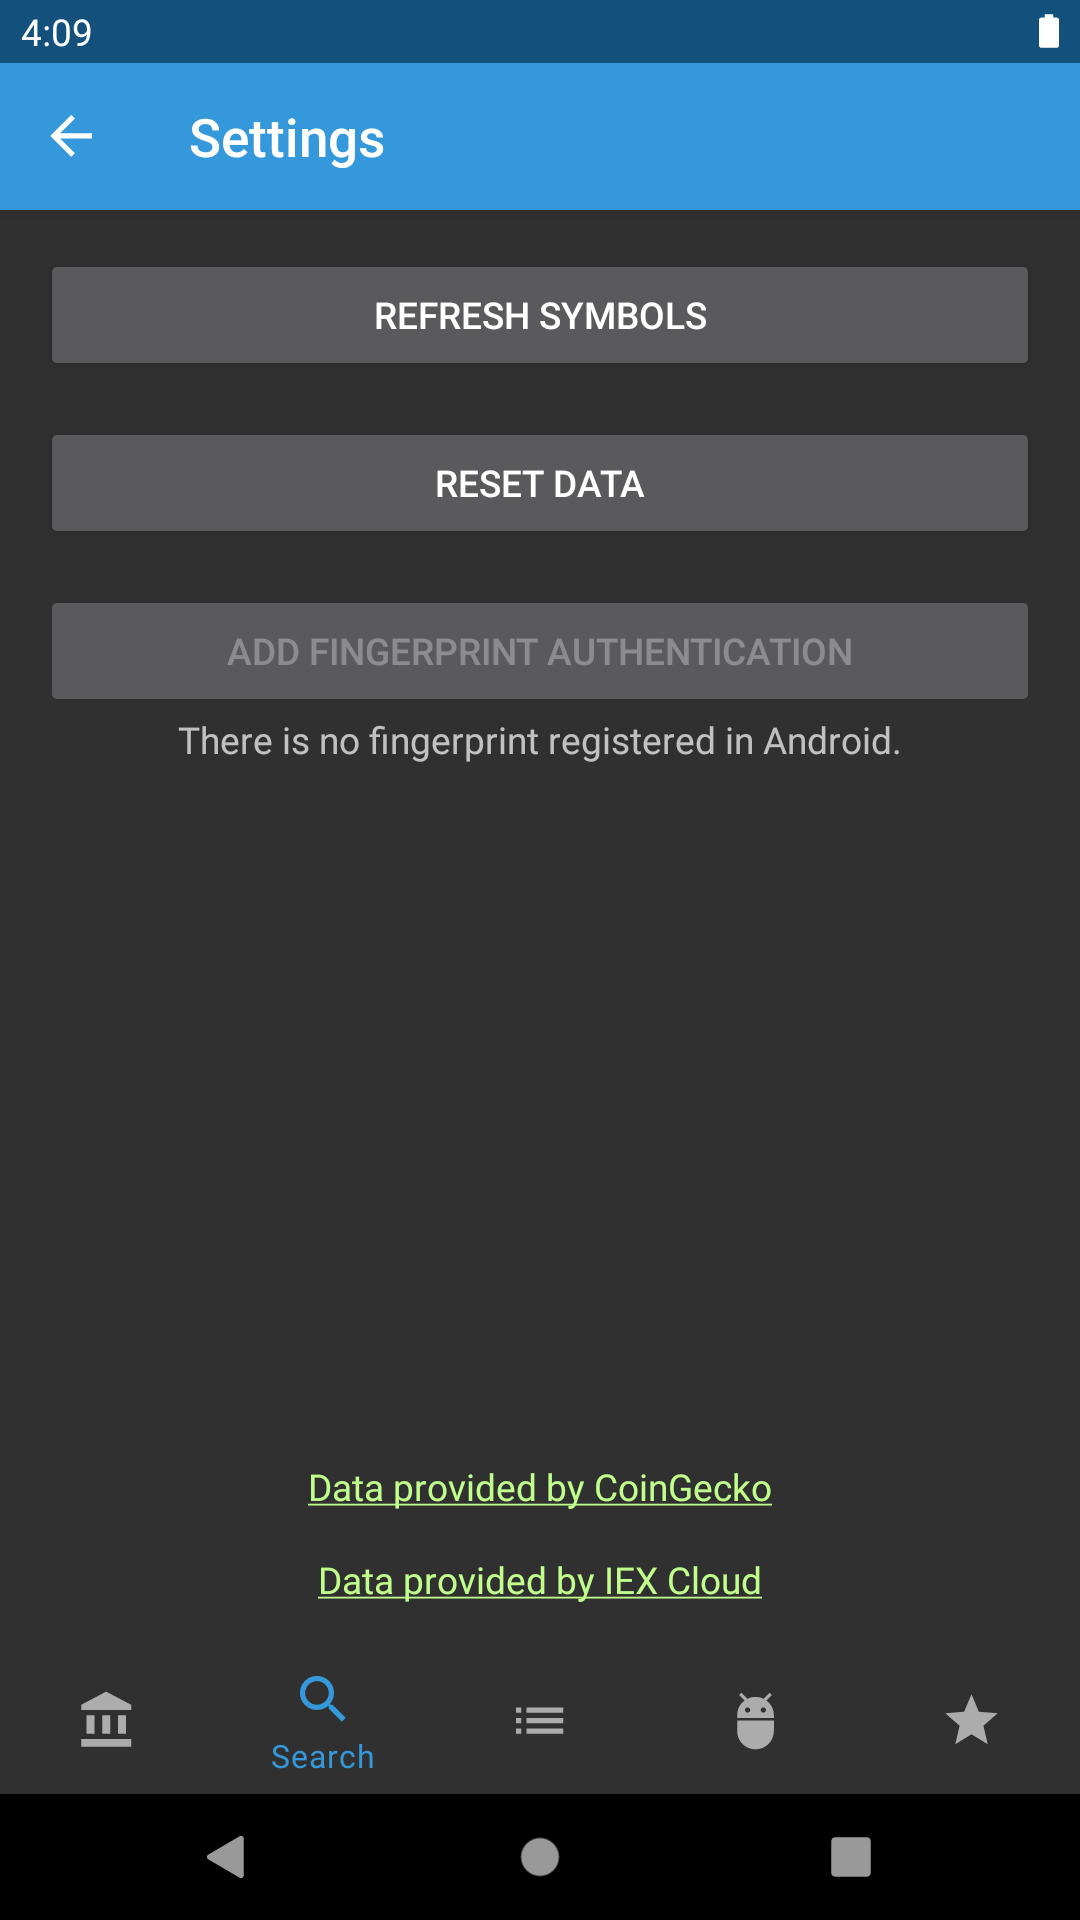
\includegraphics[height=8cm,keepaspectratio]{./images/settings/attribution.png}
		\caption{Zuschreibungen}
		\label{fig:functionality:settings:attributions}
	\end{subfigure}
	\caption{Einstellungen}
	\label{fig:functionality:settings}
\end{figure}


\section{Teamwork}
\label{sec:teamwork}
Eine Startschwierigkeit während der Zusammenarbeit war, dass nicht Entwickler im Team über ähnlich gute Kenntnisse der Android-Architektur und der Kotlin-Syntax verfügten. Dieses Problem wurde zum einen dadurch bewältigt, dass sich erfahrenere Entwickler mit den weniger erfahrenen austauschten und zu Beginn Pair-Programming \footnote{Siehe \url{https://en.wikipedia.org/wiki/Pair_programming}} machten. Durch die räumliche Zusammenarbeit und ein hohes Maß an Teamfähigkeit bei allen Teammitgliedern, konnten Probleme von Einzelnen meist schnell in der Gruppe gelöst werden. Nachdem zu Beginn Aufgaben nach technischen Schichten (Layern), wie APIs und Datenbanken vergeben wurden, gingen wir schnell dazu über, die Aufgaben nach Funktionalitäten, wie Suche, Historie, Stockbrot usw. zu vergeben. Diese Aufgabenverteilung kapselte einzelne Aufgaben wesentlich besser als die vorherige nach Schichten orientierte Aufteilung. Wir verständigten uns darauf, im Sinne der agilen Softwareentwicklung in kleinschrittigem Vorgehen Erweiterungen an einem bereits in der Frühphase funktionierenden Produkt vorzunehmen. Nach kurzem Absprache verständigten wir uns darauf, unser Projekt entsprechend dem Git-Worflow Design (Gitflow) \footnote{Siehe \url{https://www.atlassian.com/git/tutorials/comparing-workflows/gitflow-workflow}} zu versionieren. Demnach verfügte unser Projekt über zwei Haupt-Branches um den Verlauf des Projekts aufzuzeichnen. Der main-Branche enthält die offiziellen Release-Versionen des Projekts und der develop-Branche dient dazu, die einzelnen Features in ihrem zeitlichen Verlauf zu integrieren. \newline
Im Verlauf der Arbeit kristallisierten sich rasch Teamrollen heraus. Der erfahrenste Entwickler wurde schnell zum technischen Lead und Ansprechpartner bei ernsteren Problemen. Ein anderes Teammitglied ging auf den Kunden (die Aufgabenstellenden) zu um bei Unklarheiten die Aufgabenstellung zu präzisieren. Dies hat zu einem guten Arbeitsklima beigetragen. \newline
Unser Team hatte in der ganzen Woche ein positives Arbeitsklima. Jedes Teammitglied engagierte sich für das gemeinsame Ziel und trug durch kreative Ideen dazu bei, unser Projekt zu verbessern.


\section{Zusammenfassung}
\label{sec:summary}
Im Rahmen der Blockveranstaltung \textit{Code-Camp Context-Awareness 1} entwickelte unser Team ein Börsenhandelsimualtionsspiel für Android. Mit dieser Applikationen können Informationen über Aktien und Kryptowährungen abgerufen werden sowie diese als Anlagen erworben und veräußert werden. Hierbei ermöglichen eine Übersicht über das bestehende Depot, den Kontostand und alle bisherigen Transaktionen, das Spielgeschehen nachzuvollziehen. Der Handel kann durch einen Bot automatisiert werden. \newline
Bereits im Verlauf der Woche konnten wir alle gestellten Mindestanforderungen an unsere Börsenhandelsimualtion erfüllen und darüber hinaus zahlreiche zusätzliche Funkionalitäten umsetzen.


\section{Fazit}
\label{sec:conclusion}
Für die meisten Entwickler unseres Teams war dies das erste Android-Software-Projekt, wodurch die ''Lernkurve'' zu Beginn recht steil verlief. Durch unsere gute Zusammenarbeit und unseren Einsatz für das Projekt konnten wir diese Veranstaltung dazu nutzen, neue Kenntnisse der Android-Entwicklung zu erwerben und zu vertiefen. Insgesamt waren alle Teammitglieder vom Android-''Ökosystem'' positiv überrascht und fühlen uns für zukünftige App-Entwicklung gerüstet.


\section{Ausblick}
\label{sec:outlook}
% was kann man noch machen, was habt ihr nicht geschafft,..
TODO


\printbibliography[title={Referenzen}]


\pagebreak
Examples:\\

\begin{lstlisting}[caption={example kotlin code}, captionpos=b, label={lst:example}, language=Kotlin]
private suspend fun StockbrotQuote.executeSellOrder(quote: Quote) {
    val depotQuote = accountRepository.depotQuoteBySymbol(id) ?: return
    if (quote.latestPrice >= minimumSellPrice) {
        val amount = depotQuote.amount
        Timber.i("Bot is selling $amount for ${quote.latestPrice}")
        accountRepository.sell(quote, amount)
    }
}
\end{lstlisting}

\begin{figure}[H]
    \centering
    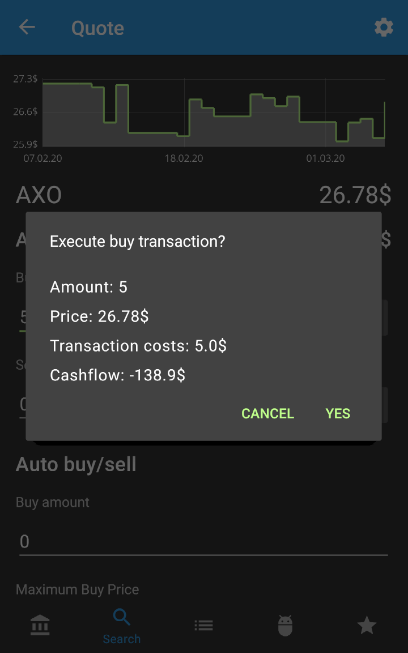
\includegraphics[height=10cm,keepaspectratio]{./images/quote_buy_confirmation_dialog.png}
    \caption{example image}
    \label{fig:example}
\end{figure}

\pagebreak


\end{document}
